\documentclass[a4paper,oneside,12pt]{book}

% KODOVANI, CESTINA
\usepackage[utf8]{inputenc}
\usepackage[czech]{babel}
\usepackage{graphicx}
\usepackage{subcaption}

\DeclareGraphicsRule{*}{mps}{*}{}

% MATEMATIKA, CITACE, ...
\usepackage{amsthm}
\usepackage{amssymb}
\usepackage{enumerate}
\usepackage{hyperref}
\usepackage{cite}
\usepackage{amsmath}

% ODKAZY
\usepackage{hyperref}

% DEFINICNI BLOK
\theoremstyle{definition}
\newtheorem{df}{Definice}
\newtheorem*{zn}{Značení}
\newtheorem*{pr}{Příklad}

\theoremstyle{plain}
\newtheorem{vt}{Věta}
\newtheorem*{tv}{Tvrzení}
\newtheorem*{pz}{Pozorování}
\newtheorem{lm}{Lemma}
\newtheorem*{hp}{Hypotéza}

\theoremstyle{remark}
\newtheorem{po}{Poznámka}

%--------------------------------------------------

\begin{document}

% ------------------------------ Titulní strana ------------------------------ %
\thispagestyle{empty}
\begin{center}
  {\Huge
  Západočeská univerzita v~Plzni\\[3pt]
  Fakulta aplikovaných věd
  }

	\vspace{10mm}

  {\Large
  \begin{tabular}{c}
		Studijní program: N1101 \\[3pt]
		Studijní obor: 1101T016 \\
  \end{tabular}
  }

  \vspace{40mm}

  {\huge \MakeUppercase{Diplomová práce}}\\[3pt]
  {\Large \textbf{Semidefinitní programování v kombinatorické optimalizaci}\par}
\end{center}

\vfill

{\large
  \begin{tabular}{ll}
    Autor: & Ondřej Špaček\\
    Vedoucí práce: & Doc. Ing. Roman Čada, Ph.D.\\[30pt]
    Plzeň, 2020 &
  \end{tabular}
}
\clearpage{\pagestyle{empty}}


% ---------------------------------- Obsah ----------------------------------- %
\tableofcontents
\setcounter{page}{1}
\pagebreak

% ----------------------------------- Úvod ----------------------------------- %
{
  \pagestyle{plain}
  \chapter*{Úvod}
\addcontentsline{toc}{chapter}{Úvod}

Matematické programování (optimalizace) se zabývá hledáním optimálních řešení matematických modelů. Modely, ve kterých se vyskytují pouze lineární funkce se zabývá lineární programování. Začátky lineárního programování jsou spojeny s druhou světovou válkou. George Dantzig, který měl na starosti vývoj logistických plánu na straně amerického letectva, v roce 1947 vymyslel Simplexovou metodu. S podobným konceptem přišel už dříve v~roce 1939 Leonid Kantorovič, ale na jeho práci bohužel nikdo nenavázal. Další slavná jména, která stojí za zmínku v souvislosti s lineárním programováním jsou John von Neumann, Albert Tucker, Harold Kuhn a spousta dalších. Relativně nová oblast optimalizace se nazývá semidefinitní programování, kterou dobře charakterizuje název článku z roku 1981 s názvem \textit{Linear Programming with Matrix Variables} od Cravena a Monda. Pokud máme optimalizační problém, ve kterém řešení jsou vyjádřena pomocí diskrétních proměnných, pak hovoříme o problému kombinatorické optimalizace. K řešení těchto problémů se v posledních cca 30 letech rozšířilo semidefinitní programování, které se využívá např. u Shannonovy kapacity grafu, studia řezů, problému obchodního cestujícího a dalších. Pro další historické informace související s optimalizací doporučuji zdroj \cite{history}, ze kterého bylo čerpáno.
  \clearpage
}


% ---------------------------- ČÁST: OPTIMALIZACE----------------------------- %
\part{Optimalizace}

\chapter{Základní geometrické pojmy}

\section{Přímky a úsečky}

Mějme dva body $x_1, x_2 \in \mathbb{R}^n$ takové, že $x_1 \neq x_2$ a parametr $\theta \in \mathbb{R}^n$. Potom výraz
\begin{equation}
    y = \theta x_1 + (1 - \theta) x_2
    \label{line}
\end{equation}
popisuje \textbf{přímku} procházející body $x_1$ a $x_2$. Pro $\theta = 0$ dostáváme bod $x_2$ a pro $\theta = 1$ bod $x_1$. Omezíme-li $\theta$ na interval $\langle 0, 1 \rangle$, dostaneme \textbf{úsečku} s koncovými body $x_1$ a $x_2$. Výraz \ref{line} lze přepsat do tvaru
$$
    y = x_2 + \theta (x_1 - x_2),
$$
který můžeme interpretovat jako součet počátečního bodu $x_2$ a nějakého násobku směrového vektoru $x_1 - x_2$.

\section{Afinní prostory}

Říkáme, že $C \subseteq \mathbb{R}^n$ je \textbf{afinní prostor}, jestliže přímka procházející libovolnými dvěma různými body z $C$ leží v $C$. Tedy $C$ obsahuje lineární kombinace libovolných dvou bodů z $C$, jestliže součet koeficientů lineární kombinace je roven jedné. To lze zobecnit i pro více než dva body. Lineární kombinace $\theta_1 x_1 + \dots + \theta_k x_k$ bodů $x_1, \dots, x_k$ taková, že $\theta_1 + \dots + \theta_k = 1$, se nazývá \textbf{afinní kombinace} bodů $x_1, \dots, x_k$. Indukcí z definice afinního prostoru lze snadno ukázat, že pokud $C$ je afinní množina, $x_1, \dots, x_k \in C$ a $\theta_1 + \dots + \theta_k = 1$, potom bod $\theta_1 x_1 + \dots + \theta_k x_k \in C$.

\noindent Nechť $C$ je afinní prostor a $x_0 \in C$, potom množina
$$
    V = C - x_0 = \left\{ x - x_0 \mid c \in C \right\}
$$
je \textbf{vektorový prostor}, tj. množina, která je uzavřená na sčítání a násobení skalárem.

\noindent Afinní prostor $C$ lze vyjádřit jako
$$
    C = V + x_0 = \left\{ v + x_0 \mid v \in V \right\},
$$
kde $V$ je vektorový prostor a $x_0$ je počátek. Poznamenejme, že vektorový prostor $V$ asociovaný s afinním prostorem $C$ nezávisí na volbě počátku $x_0$.

\noindent \textbf{Dimenze} afinního prostoru $C = V + x_0$ je definována jako dimenze vektorového prostoru $V = C - x_0$, kde $x_0$ je libovolný prvek z $C$. Množina všech afinních kombinací bodů množiny $C \subseteq \mathbb{R}^n$ se nazývá \textbf{afinní obal} množiny $C$. Afinní obal množiny $C$ budeme značit
$$
    \textbf{aff } C = \left\{ \theta_1 x_1 + \dots + \theta_k x_k \mid x_1, \dots, x_k \in C, \theta_1 + \dots + \theta_k = 1 \right\}.
$$
Afinní obal je nejmenší afinní prostor, který obsahuje množinu $C$. Tedy, jestliže $S$ je afinní prostor takový, že $C \subseteq S$, potom $\textbf{aff }C \subseteq S$.


\section{Konvexní množiny}

Říkáme, že množina $C$ je \textbf{konvexní}, jestliže úsečka mezi libovolnými dvěma body z $C$ leží také v $C$. Jinak řečeno, jestliže pro libovolné dva body $x_1, x_2 \in C$ a libovolné $\theta \in \langle 0, 1 \rangle$ platí, že $\theta x_1 + (1 - \theta) x_2 \in C$. Poznamenejme, že každý afinní prostor je zároveň konvexní množinou. Podobně jako afinní kombinaci definujeme \textbf{konvexní kombinaci} bodů $x_1, \dots, x_k$ jako $\theta_1 x_1 + \dots + \theta_k x_k$, kde $\theta_1 + \dots + \theta_k = 1, \theta_i \geq 0$ pro $i = 1, \dots, k$. \textbf{Konvexní obal} množiny $C$ je množina všech konvexních kombinací bodů z množiny $C$, značíme
$$
    \textbf{conv }C = \left\{ \theta_1 x_1 + \dots + \theta_k x_k \mid x_i \in C, \theta_i \geq 0, i = 1, \dots, k, \theta_1 + \dots + \theta_k = 1 \right\}.
$$
Analogicky, konvexní obal množiny $C$ je nejmenší konvexní množina, která obsahuje množinu $C$. Pro představu viz obrázek~\ref{fig:convex_hull}.

\begin{figure}[h!]
    \centering
    \begin{subfigure}[b]{0.3\textwidth}
        \centering
        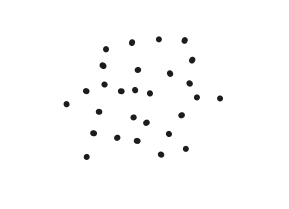
\includegraphics[width=\textwidth]{img/points_for_convex_hull.png}
        \caption{Množina bodů $C$}
        \label{fig:convex_hull:a}
    \end{subfigure}

    \hfill

    \begin{subfigure}[b]{0.3\textwidth}
        \centering
        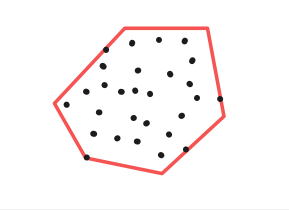
\includegraphics[width=\textwidth]{img/convex_hull.png}
        \caption{$\textbf{conv }C$}
        \label{fig:convex_hull:b}
    \end{subfigure}
     
    \caption{Konvexní obal množiny}
    \label{fig:convex_hull}
\end{figure}


\section{Kužely}

Množina $C$ se nazývá \textbf{kužel}, jestliže pro každé $x \in C$ a $\theta \geq 0$ platí, že $\theta x \in C$. Je-li $C$ navíc konvexní, pak se $C$ nazývá \textbf{konvexní kužel}. Tedy $C$ je konvexní kužel, jestliže pro libovolné $x_1, x_2 \in C$ a $\theta_1, \theta_2 \geq 0$ platí, že $\theta_1 x_1 + \theta_2 x_2 \in C$. Říkáme, že bod ve tvaru $\theta_1 x_1 + \dots + \theta_k x_k$, kde $\theta_1, \dots, \theta_k \geq 0$ je \textbf{kuželovou kombinací} bodů $x_1, \dots, x_k$. Dále, pokud $x_i$ leží v konvexním kuželu množiny $C$, potom libovolná kuželová kombinace bodu $x_i$ leží rovněž v konvexním kuželu množiny $C$. Platí, že množina $C$ je konvexní kužel právě tehdy, když $C$ obsahuje všechny kuželové kombinace svých bodů. \textbf{Kuželový obal} množiny $C$ je množina, která obsahuje všechny kuželové kombinace množiny $C$, tj.
$$
    \textbf{cone }C = \left\{ \theta_1 x_1 + \dots + \theta_k x_k \mid x_i \in C, \theta_i \geq 0, i = 1, \dots, k \right\}.
$$
Kuželový obal množiny $C$ je zároveň nejmenší konvexní kužel, který obsahuje množinu $C$. Pro představu viz obrázek~\ref{fig:cone_hull}.

\begin{figure}[h!]
    \centering
    \begin{subfigure}[b]{0.3\textwidth}
        \centering
        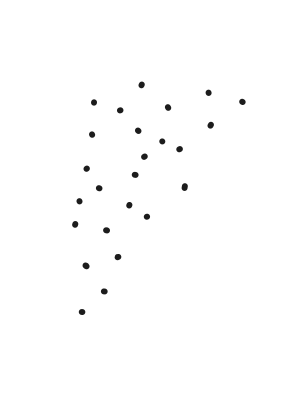
\includegraphics[width=\textwidth]{img/points_for_cone_hull.png}
        \caption{Množina bodů $C$}
        \label{fig:cone_hull:a}
    \end{subfigure}

    \hfill

    \begin{subfigure}[b]{0.3\textwidth}
        \centering
        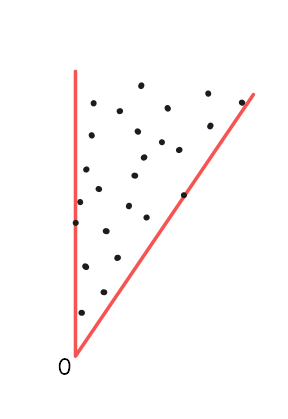
\includegraphics[width=\textwidth]{img/cone_hull.png}
        \caption{$\textbf{cone }C$}
        \label{fig:cone_hull:b}
    \end{subfigure}
     
    \caption{Kuželový obal množiny}
    \label{fig:cone_hull}
\end{figure}

\section{Nadroviny a poloprostory}

\textbf{Nadrovina} je množina ve tvaru
$$
    \left\{ x \mid a^T x = b \right\},
$$
kde $a \in \mathbb{R}^n$, $a \neq 0$ a $b \in \mathbb{R}$. Analyticky se na nadrovinu koukáme jako na množinu všech řešení netriviální lineární rovnice. Geometricky zase jako na množinu všech bodů takových, že mají konstantní skalární součin s normálovým vektorem $a$. Konstanta $b$ značí posunutí nadroviny od počátku. Nadrovinu také můžeme vyjádřit jako
$$
    \left\{ x \mid a^T (x - x_0) = 0 \right\} = x_0 + \left\{ v \mid a^T v = 0 \right\},
$$
kde $x_0$ je libovolný bod této nadroviny a $\left\{ v \mid a^T v = 0 \right\}$ je množina všech vektorů, které jsou kolmé k normálovému vektoru $a$. Nadrovina je tedy množina, která obsahuje bod $x_0$ a libovolný bod ve tvaru $x_0 + v$, kde $v$ je vektor, který je kolmý k normálovému vektoru $a$. Pro ilustraci v $\mathbb{R}^2$ viz obrázek~\ref{fig:hyperplane}.

Nadrovina dělí $\mathbb{R}^n$ na dva poloprostory. Množina 
$$
    \left\{ x \mid a^T x \leq b \right\}, \text{ resp. } \left\{ x \mid a^T x < b \right\},
$$
kde $a \neq 0$ se nazývá (uzavřený) \textbf{poloprostor}, resp. \textbf{otevřený poloprostor}. Je to tedy množina všech řešení netriviální lineární nerovnice. Podobně jako nadrovinu, můžeme poloprostor vyjádřit ve tvaru
$$
    \left\{ x \mid a^T (x - x_0) \leq 0 \right\}, \text{ resp. } \left\{ x \mid a^T (x - x_0) < 0 \right\},
$$
kde $a \neq 0$ a $x_0$ je libovolný bod z nadroviny $\left\{ x \mid a^T x = b \right\}$. Poloprostor tedy obsahuje bod $x_0$ a libovolný bod $x_0 + v$, kde $v$ je vektor, který s vnějším normálovým vektorem svírá tupý nebo pravý úhel. Tato interpretace je v $\mathbb{R}^2$ ilustrována na obrázku~\ref{fig:halfspace}. Ještě poznamenejme, že poloprostory jsou konvexní množiny, ale samozřejmě nejsou afinní.

\begin{figure}[h!]
    \centering
    \begin{subfigure}[b]{0.3\textwidth}
        \centering
        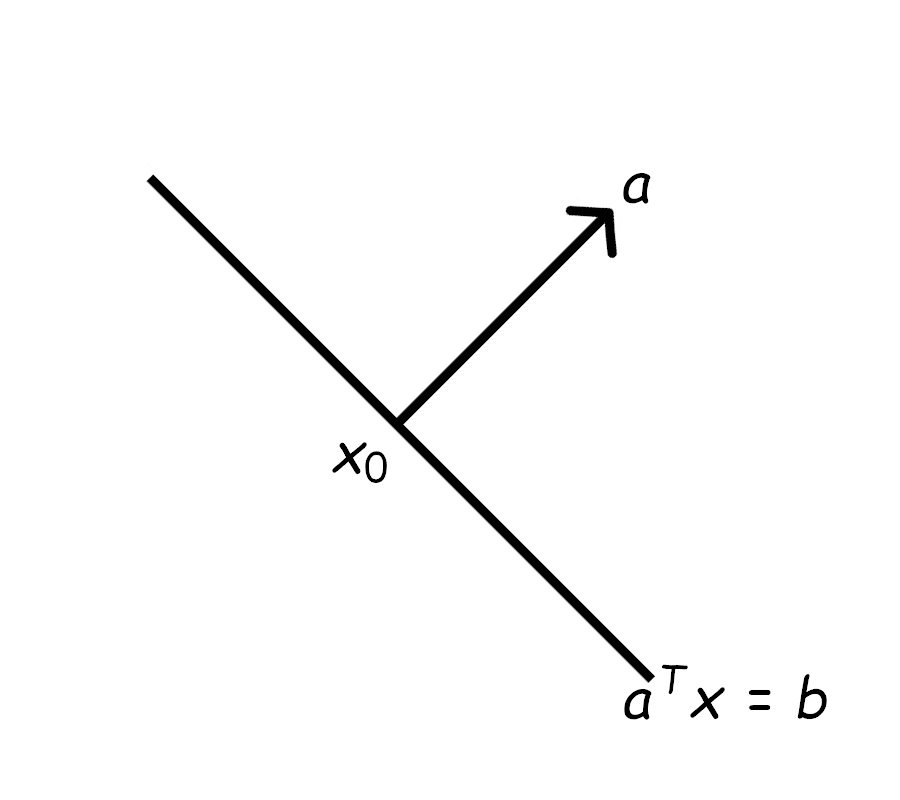
\includegraphics[width=\textwidth]{img/hyperplane.jpg}   
        \caption{Nadrovina}
        \label{fig:hyperplane}
    \end{subfigure}

    \hfill

    \begin{subfigure}[b]{0.3\textwidth}
        \centering
        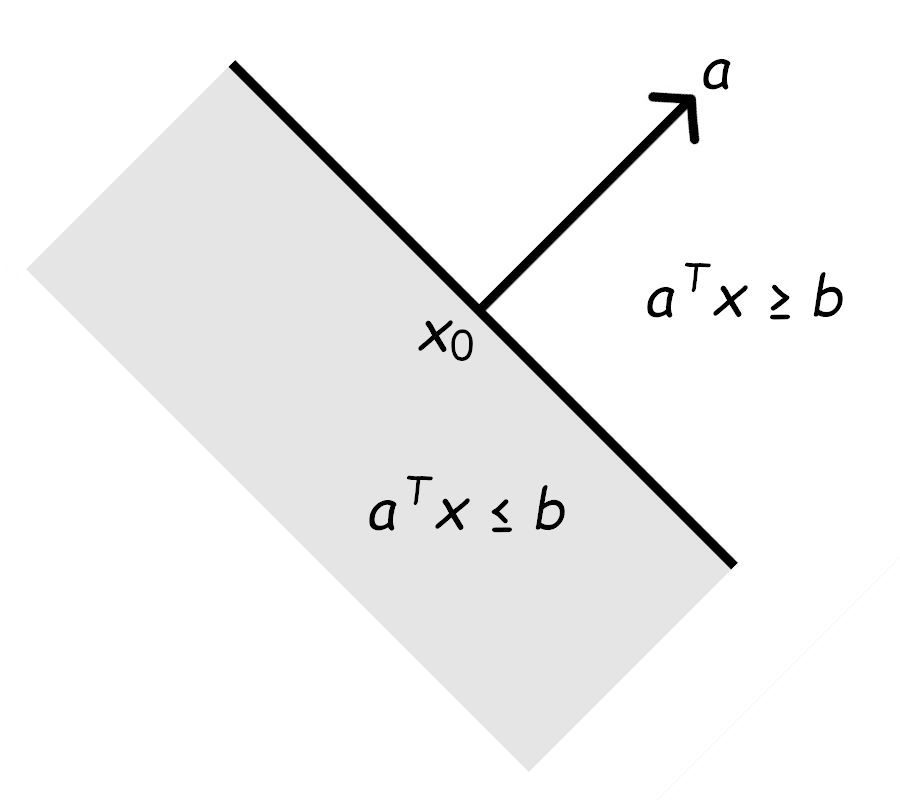
\includegraphics[width=\textwidth]{img/halfspace.jpg}   
        \caption{Poloprostor}
        \label{fig:halfspace}
    \end{subfigure}

    \caption{Nadrovina a poloprostor v $\mathbb{R}^2$.}
    \label{fig:hyperplane_halfspace}
\end{figure}

\section{Polyedry a polytopy -- PŘEPSAT / DOPLNIT}

Mějmě konečně mnoho uzavřených poloprostorů v $\mathbb{R}^n$. Množina, která vznikne jejich průnikem se nazývá \textbf{polytop}. Je-li navíc polytop omezený, potom ho nazýváme \textbf{polyedr}. Polyedr lze také ekvivalentně definovat jako konvexní obal konečně mnoha bodů v $\mathbb{R}^n$. Důležitý fakt říká Minkowského-Weyleova věta.
%Příkladem polyedrů v $\mathbb{R}^3$ jsou např. platónská tělesa, viz obrázek~\ref{fig:platon_solids}. 

\begin{vt}[Minkowski-Weyl]
    TODO
\end{vt}

%každý polytop $P$ je konečně generovaný a můžeme ho vyjadřit jako
%$$
%    P = \textbf{conv }(u_1, \dots, u_r) + \textbf{cone }(v_1, \dots, v_s),
%$$
%kde $u_i, v_i$ jsou extremální vrcholy $P$.

%\begin{figure}[h!]
%    \centering
%    \begin{subfigure}[b]{0.3\textwidth}
%        \centering
%        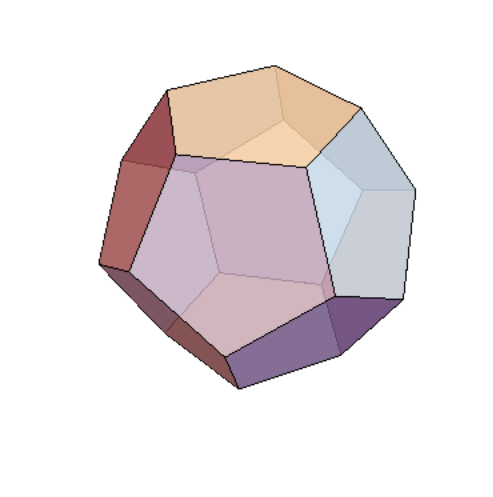
\includegraphics[width=\textwidth]{img/dodecahedron.png}   
%        \caption{Dodecahedron.}
%    \end{subfigure}
%
%    \hfill
%
%    \begin{subfigure}[b]{0.3\textwidth}
%        \centering
%        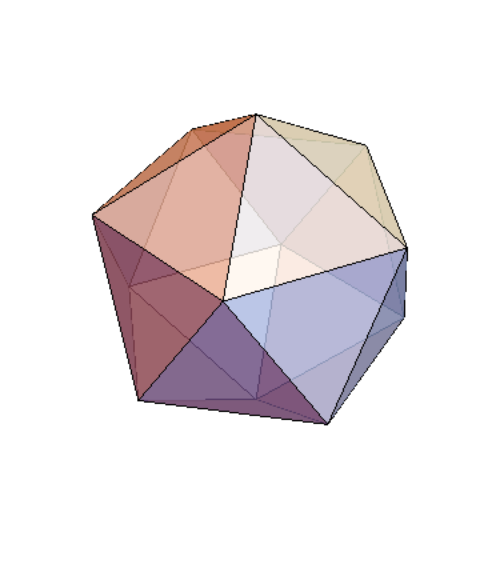
\includegraphics[width=\textwidth]{img/icosahedron.png}   
%        \caption{Icosahedron.}
%    \end{subfigure}
%
%        \begin{subfigure}[b]{0.3\textwidth}
%        \centering
%        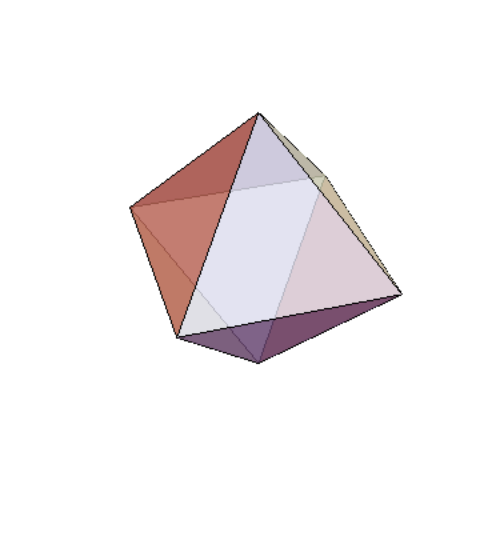
\includegraphics[width=\textwidth]{img/octahedron.png}   
%        \caption{Octahedron.}
%    \end{subfigure}
%
%    \caption{Platónská tělesa.}
%    \label{fig:platon_solids}
%\end{figure}
\clearpage

\chapter{Konvexní optimalizace}

Kapitola je zpracována z \textbf{[REF]}, \textbf{[REF]}, ...

\section{Obecná podmíněná úloha}

\begin{equation}\label{eq:constrained_problem}
    \begin{split}
        &\inf\ f(x) \\
        &g_i(x) \leq 0, i = 1, \dots, m \\
        &h_i(x) = 0, i = 1, \dots, p
    \end{split}
\end{equation}

Hledáme $x \in \mathbb{R}^n$, které minimalizuje $f(x)$, vzhledem k omezením $g_i(x)$ a $h_i(x)$. Proměnné $x$ říkáme \textbf{optimalizační proměnná}, funkci $f(x)$ říkáme \textbf{cenová} nebo \textbf{účelová funkce}. Výrazy $g_i(x) \leq 0$ jsou \textbf{omezení typu nerovnosti} a $h_i(x) = 0$ jsou \textbf{omezení typu rovnosti}. Říkáme, že problém~\ref{eq:constrained_problem} je \textbf{úloha nepodmíněné optimalizace}, jestliže $m = p = 0$. Jinak se jedná o \textbf{úlohu podmíněné optimalizace}.

\textbf{Definiční obor} $\mathcal{D}$ úlohy~\ref{eq:constrained_problem} je
$$
    \mathcal{D} = \bigcap_{i=1}^m \textbf{dom}\ g_i \cap \bigcap_{i=1}^p \textbf{dom}\ h_i.
$$
Říkáme, že bod $x \in \mathcal{D}$ je \textbf{přípustný}, jestliže splňuje všechna omezení $g_i(x) \leq 0$ a $h_i(x) = 0$. Úloha~\ref{eq:constrained_problem} je \textbf{přípustná}, jestliže existuje alespoň jeden bod $x \in \mathcal{D}$, který je přípustný. Množina všech přípustných bodů $x \in \mathcal{D}$ se nazývá \textbf{přípustná množina}.

\textbf{Optimální hodnota} $f^*$ úlohy~\ref{eq:constrained_problem} je definována jako
$$
    f^* = \inf \left\{ f(x) \mid g_i(x) \leq 0, i = 1, \dots, m, h_i(x) = 0, i = 1, \dots, p \right\}.
$$

\section{Konvexní podmíněná úloha}

\begin{equation}\label{eq:convex_problem}
    \begin{split}
        &\inf\ f(x) \\
        &g_i(x) \leq 0, i = 1, \dots, m \\
        &a_i^Tx = b_i, i = 1, \dots, p
    \end{split}
\end{equation}

Oproti obecné úloze~\ref{eq:constrained_problem} jsou funkce $f(x), g_i(x)$ konvexní a funkce $h_i(x) = a_i^Tx - b_i$ jsou afinní. Přípustná množina takové úlohy je konvexní množinou.

\section{Lagrangeova dualita}

Mějme úlohu~\ref{eq:constrained_problem} s $\mathcal{D} \neq \emptyset$. Zobrazení $L:\ \mathbb{R}^n \times \mathbb{R}^m \times \mathbb{R}^p \rightarrow \mathbb{R}$ takové, že
\begin{equation}
    L(x, \lambda, \mu) = f(x) + \sum_{i=1}^m \lambda_i g_i(x) + \sum_{i=1}^p \mu_i h_i(x)
\end{equation}
se nazývá \textbf{Lagrangeova funkce}. Definiční obor $\textbf{dom}\ L = \mathcal{D} \times \mathbb{R}^m \times \mathbb{R}^p$. Vektory $\lambda = (\lambda_1, \dots, \lambda_m)$ a $\mu = (\mu_1, \dots, \mu_p)$ nazýváme \textbf{duální proměnné} a prvkům těchto vektorů říkáme \textbf{Lagrangeovy multiplikátory}. Dále definujeme \textbf{duální funkci}
$$
    d:\ \mathbb{R}^m \times \mathbb{R}^p \rightarrow \mathbb{R}
$$
jako infimum Lagrangeovy funkce $L$ přes všechna $x \in \mathcal{D}$. Tedy
\begin{equation}
    d(\lambda, \mu) = \inf_{x \in \mathcal{D}} L(x, \lambda, \mu) = \inf_{x \in \mathcal{D}} \left( f(x) + \sum_{i=1}^m \lambda_i g_i(x) + \sum_{i=1}^p \mu_i h_i(x) \right).
\end{equation}

Poznamenejme, že duální funkce je konkávní bez ohledu na to, zda je úloha konvexní a je-li $L$ zdola neomezená v proměnné $x$, potom duální funkce nabývá hodnoty $-\infty$.

\subsection*{Dolní odhad na $f^*$}\label{s:lower_bound}

Nechť $\tilde{x}$ je přípustný bod. Pro $\lambda \geq 0$ je
$$
    \sum_{i=1}^m \lambda_i g_i(\tilde{x}) + \sum_{i=1}^p \mu_i h_i(\tilde{x}) \leq 0.
$$
Potom pro Lagrangeovu funkci můžeme psát
$$
    L(\tilde{x}, \lambda, \mu) = f(\tilde{x}) + \sum_{i=1}^m \lambda_i g_i(\tilde{x}) + \sum_{i=1}^p \mu_i h_i(\tilde{x}) \leq f(\tilde{x}).
$$
A tedy pro duální funkci platí
$$
    d(\lambda, \mu) = \inf_{x \in \mathcal{D}} L(x, \lambda, \mu) \leq L(\tilde{x}, \lambda, \mu) \leq f(\tilde{x}).
$$

\subsection*{Duální úloha}

V části~\ref{s:lower_bound} jsme si ukázali, že duální funkce dává dolní odhad na optimální hodnotu $x^*$ úlohy~\ref{eq:constrained_problem}. Stále jsme si ale neřekli, jaký je nejlepší dolní odhad, který pomocí duální funkce jsme schopni dostat. To nás dostává k následující optimalizační úloze.
\begin{equation}\label{eq:dual_problem}
    \begin{split}
        &\sup d(\lambda, \mu) \\
        &\lambda \geq 0
    \end{split}
\end{equation}

Úloze~\ref{eq:dual_problem} se říká \textbf{Lagrangeova duální úloha} příslušná k úloze~\ref{eq:constrained_problem}, kterou nazýváme \textbf{primární úlohou}.

\subsection*{Slabá dualita}

Optimální řešení Lagrangeovy duální úlohy označíme $d^*$, které je už z definice nejlepší dolní odhad na optimální řešení primární úlohy $f^*$. Tato nerovnost platí i pokud primární úloha není konvexní. Této nerovnosti říkáme \textbf{slabá dualita}. Rozdíl optimálních řešení $f^* - d^*$ označujeme jako \textbf{optimální dualitní rozdíl} primární úlohy. Poznamenejme, že optimální dualitní rozdíl je vždy nezáporný.


\subsection*{Silná dualita a Slaterova podmínka}

Pokud je optimální dualitní rozdíl $f^* - d^* = 0$, pak říkáme, že platí silná dualita. Silná dualita obecně neplatí, ale pro primární úlohu, která splňuje nějaké další podmínky to možné je. Těmto podmínkám se říká \textbf{podmínky kvalifikace omezení}. Jednou takovou je \textbf{Slaterova podmínka}
$$
    \exists x \in \textbf{relint}\ \mathcal{D}:\ g_i(x) < 0, i = 1, \dots, m, Ax = b.
$$

Bodu $x \in \mathcal{D}$, který splňuje Slaterovu podmínku, říkáme, že je \textbf{striktně přípustný}, protože omezení typu nerovnosti jsou ostré. Pokud jsou některé funkce $g_i$ afinní, můžeme Slaterovu podmínku modifikovat. Nechť tedy $g_1, \dots, g_k, k \leq m$, jsou afinní funkce. Potom \textbf{modifikovaná Slaterova podmínka} má tvar
$$
    \exists x \in \textbf{relint}\ \mathcal{D}:\ g_i(x) \leq 0, i = 1, \dots, k, g_i(x) < 0, i = k+1, \dots, m, Ax = b.
$$

\noindent Pro úlohu~\ref{eq:convex_problem} platí následující věta.
\begin{vt2}[Slaterova]
    Nechť primární úloha je konvexní a platí (modifikovaná) Slaterova podmínka, potom $f^* = d^*$.
\end{vt2}


%\section*{TODO}
%\textbf{Použití duální úlohy:} obecnou primární úlohu je těžké vyřešit, ale duální úloha je vždy konvexní, tak vyřeším tu a mám alespoň dolní odhad na primární úlohu

\clearpage

\chapter{Lineární programování}

\section{Primární úloha}

Úlohou lineárního programování rozumíme minimalizaci nebo maximalizaci lineární \textbf{účelové funkce} vzhledem k afinním \textbf{omezením}, kde tato omezení jsou dána soustavou lineární rovnic a nerovnic. Úlohu lineárního programování lze formulovat v několika ekvivalentních tvarech, které se liší zadáním omezení. Úloha v \textbf{kanonickém tvaru} má svá omezení dána soustavou lineárních nerovnic $Ax \leq b$. Tedy
\begin{equation}\tag{LP-P}
    \max \left\{ c^T x \mid Ax \leq b, x \geq 0 \right\},
    \label{eq:LP-P}
\end{equation}
kde $A \in \mathbb{R}^{m \times n}$, $b \in \mathbb{R}^n$, $x \in \mathbb{R}^n$ a $c \in \mathbb{R}^n$. \textbf{Přípustná množina řešení} je průnikem poloprostorů, které jsou definovány soustavou nerovnic $Ax \leq b$ a \textbf{nezáporného ortantu}, tj. množiny $\left\{ x \in \mathbb{R}^n \mid x_i \geq 0, i = 1, \dots, n \right\}$. Obě tyto množiny jsou konvexní a tedy i jejich průnik je rovněž konvexní množina. Dále, protože přípustnou množinu máme popsanou soustavou konečně mnoha lineárních nerovnic, geometricky se na úlohu \ref{eq:LP-P} díváme jako na maximalizaci lineární funkce přes polyedr, který je definován touto soustavou.

\begin{pr}
Mějme následující maximalizační úlohu.
\begin{equation}\tag{P1}
    \begin{split}
        \max x_1 + x_2 &       \\
        - x_1 + 3 x_2  &\leq 4 \\
        4 x_1 -   x_2  &\leq 6 \\
        x &\geq 0.
    \end{split}
    \label{eq:P1}
\end{equation}

Přípustná množina řešení je zobrazena na obrázku~\ref{fig:ex1}. Řešením úlohy je vektor $x^* = (2, 2)$ s cenou $4$. Implementace v softwaru MOSEK: \url{https://github.com/c0n73x7/D1PL0MK4/blob/master/mosek/ex1.py}.
\end{pr}

\begin{figure}[h!]
    \centering
    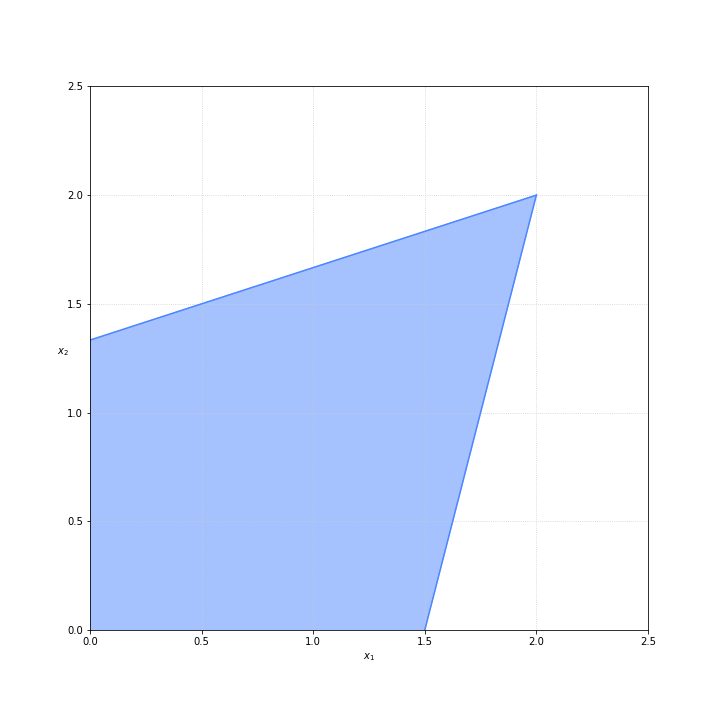
\includegraphics[width=0.5\textwidth]{img/ex1.png}   
    \caption{Přípustná množina řešení k úloze~\ref{eq:P1}.}
    \label{fig:ex1}
\end{figure}

\section{Dualita}

Pomocí Lagrangeovy duality odvodíme duální úlohu k primární úloze~\ref{eq:LP-P}. Máme tedy optimalizační úlohu
\begin{equation*}
    \min \left\{ -c^Tx \mid Ax \leq b, x \geq 0 \right\}.
\end{equation*}

\noindent Pro ní vytvoříme Lagrangeovu funkci
\begin{equation*}
    \begin{split}
        L(x, \lambda) &= -c^Tx + \lambda^T \left( Ax - b \right) - \lambda^Tx \\
                      &= -b^T\lambda + \left( A^T\lambda - c - \lambda \right)^Tx.
    \end{split}
\end{equation*}

\noindent Z Lagrangeovy funkce přejdeme k duální funkci
\begin{equation*}
    \begin{split}
        d(\lambda)  &= \inf_x L(x, \lambda) \\
                    &= \inf_x -b^T\lambda + \left( A^T\lambda - c - \lambda \right)^Tx \\
                    &=
                    \begin{cases}
                        -b^T\lambda & \text{pokud } A^T\lambda - c - \lambda = 0, \\
                        -\infty     & \text{jinak}.
                    \end{cases}
    \end{split}
\end{equation*}

\noindent Tu nakonec použijeme v duální úloze
\begin{equation*}
    \max \left\{ -b^T\lambda \mid A^T\lambda -c - \lambda = 0 \right\}
\end{equation*}

\begin{equation*}
    \max \left\{ -b^T\lambda \mid A^T\lambda \geq c, \lambda \geq 0 \right\}
\end{equation*}

\begin{equation}\tag{LP-D}
    \min \left\{ b^T\lambda \mid A^T\lambda \geq c, \lambda \geq 0 \right\}
    \label{eq:LP-D}
\end{equation}

\noindent Dostáváme tedy duální úlohu~\ref{eq:LP-D} k primární úloze~\ref{eq:LP-P}.

\begin{pr}
Duální úloha k \ref{eq:P1} je v následujícím tvaru.
\begin{equation}\tag{P2}
    \begin{split}
        \min 4 y_1 + 6 y_2 &       \\
        - y_1 + 4 y_2      &\geq 1 \\
        3 y_1 -   y_2      &\geq 1 \\
        y &\geq 0.
    \end{split}
    \label{eq:P2}
\end{equation}

Přípustná množina řešení je zobrazena na obrázku~\ref{fig:ex2}. Řešením úlohy je vektor $y^* \approx (0.4546, 0.3636)$ s cenou $4$. Implementace v softwaru MOSEK: \url{https://github.com/c0n73x7/D1PL0MK4/blob/master/mosek/ex2.py}.
\end{pr}

\begin{figure}[h!]
    \centering
    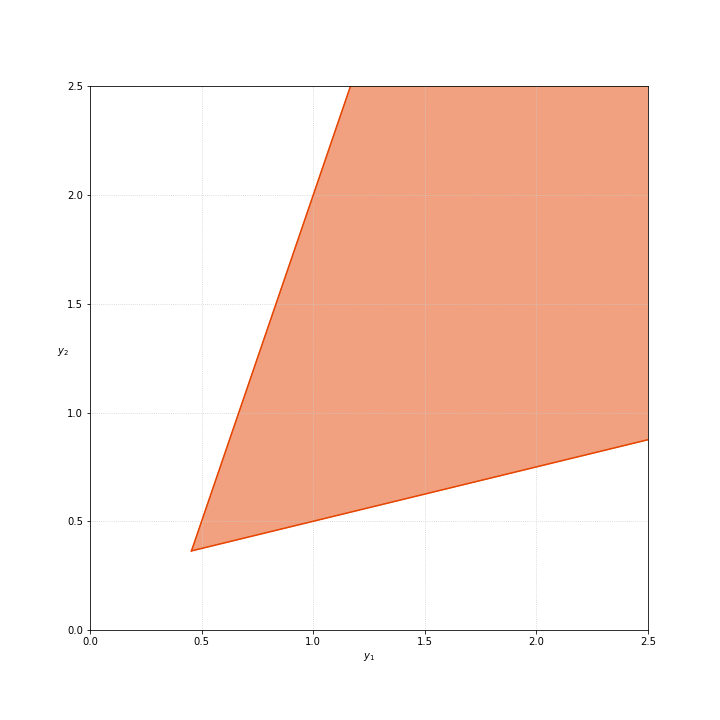
\includegraphics[width=0.5\textwidth]{img/ex2.png}   
    \caption{Přípustná množina řešení k úloze~\ref{eq:P2}.}
    \label{fig:ex2}
\end{figure}

Všimněme si, že v příkladech \ref{eq:P1} a \ref{eq:P2} mají řešení $x^*$ i $y^*$ stejnou cenu. To není náhoda a tento fakt je obsahem silné věty o dualitě lineárního programování, kterou dokázal v roce 1947 John von Neumann. Začneme slabou větou o dualitě lineárního programování.

\begin{vt2}[Slabá věta o dualitě.]
    Nechť $\tilde{x}$ je přípustné řešení \ref{eq:LP-P} a $\tilde{y}$ je přípustné řešení \ref{eq:LP-D}. Potom $c^T \tilde{x} \leq b^T \tilde{y}$.
\end{vt2}

Tedy každé přípustné řešení $\tilde{y}$ duální úlohy \ref{eq:LP-D} nám dává horní odhad na maximum účelové funkce primární úlohy \ref{eq:LP-P}. Graficky můžeme slabou větu o dualitě interpretovat jako na obrázku~\ref{fig:weak_duality}. Zatím tedy nevíme, zda vždy existují přípustná (optimální) řešení $x^*$ pro úlohu \ref{eq:LP-P} a $y^*$ pro úlohu \ref{eq:LP-D}, pro která platí $c^T x^* = b^T y^*$. Kladnou odpověď dostaneme z již zmíněné silné věty od dualitě.

\begin{figure}[h!]
    \centering
    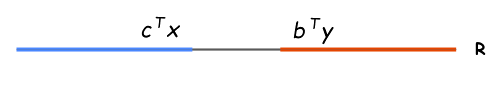
\includegraphics[width=0.5\textwidth]{img/weak_duality.png}   
    \caption{Slabá věta o dualitě.}
    \label{fig:weak_duality}
\end{figure}

\begin{vt2}[Silná věta o dualitě.]
    Jestliže úlohy \ref{eq:LP-P} a \ref{eq:LP-D} mají přípustná řešení. Potom
    $$
        \max \left\{ c^T x \mid Ax \leq b, x \geq 0 \right\} = \min \left\{ b^T y \mid A^T y \geq c, y \geq 0 \right\}.
    $$ 
\end{vt2}
Se znalostí silné věty o dualitě můžeme obrázek~\ref{fig:weak_duality} upravit na obrázek~\ref{fig:strong_duality}.

\begin{figure}[h!]
    \centering
    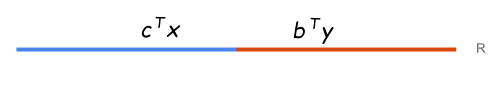
\includegraphics[width=0.5\textwidth]{img/strong_duality.png}
    \caption{Ceny přípustných řešení primární a příslušné duální úlohy.}
    \label{fig:strong_duality}
\end{figure}

\section{Komplementární skluzovost}

Pro odvození tzv. podmínky komplementární skluzovosti nejprve převedeme úlohy \ref{eq:LP-P} a \ref{eq:LP-D} do jiných tvarů. V primární úloze povolíme $x \in \mathbb{R}^n$. Tedy primární úloha je ve tvaru

\begin{equation}\tag{LP-P2}
    \max \left\{ c^T x \mid Ax \leq b \right\}.
    \label{eq:LP-P2}
\end{equation}
A příslušná duální úloha je ve tvaru

\begin{equation}\tag{LP-D2}
    \min \left\{ b^T y \mid A^T y = c, y \geq 0 \right\}.
    \label{eq:LP-D2}
\end{equation}

Nechť $\tilde{x}$ je připustné řešení a $x^*$ je optimální řešení úlohy \ref{eq:LP-P2}, $\tilde{y}$ je přípustné řešení a $y^*$ je optimální řešení úlohy \ref{eq:LP-D2}. \textbf{Dualitní rozdíl} $\tilde{x}$ a $\tilde{y}$ je číslo $b^T \tilde{y} - c^T \tilde{x} \geq 0$. Ze silné věty o dualitě samozřejmě plyne, že pro optimální řešení $x^*$ a $y^*$ je dualitní rozdíl roven $0$. Vyjdeme z dualitního rozdílu optimálních řešení.
$$
    b^T y^* - c^T x^* = y^{*^T} b - y^{*^T} A x^* = y^{*^T} \left( b - A x^* \right) = 0.
$$
Poslední rovnost přepíšeme maticově
$$
    \left[ y_1^*, \dots, y_m^* \right] \left(
        \begin{bmatrix}
            b_1    \\
            \vdots \\
            b_m
        \end{bmatrix}
        -
        \begin{bmatrix}
            a_{11} & \dots & a_{1n} \\
            \vdots & \     & \vdots \\
            a_{m1} & \dots & a_{mn}
        \end{bmatrix}
        \begin{bmatrix}
            x_1^*  \\
            \vdots \\
            x_n^*
        \end{bmatrix}
    \right)
    =
    \begin{bmatrix}
    0      \\
    \vdots \\
    0
    \end{bmatrix}.
$$
Dostáváme tedy soustavu rovnic $y_i^* \left( b_i - a_{i\_} x^* \right) = 0$, kde $i = 1, \dots, m$. Tedy buď $y_i^* = 0$ nebo $ b_i - a_{i\_} x^* = 0$. \textbf{Podmínka komplementární skluzovosti} je splněna, jestliže pro přípustná řešení $\tilde{x}, \tilde{y}$ platí buď $\tilde{y}_i = 0$ nebo $b_i - a_{i\_} \tilde{x} = 0$, $i = 1, \dots, m$. Pokud nastane $b_i - a_{i\_} \tilde{x} = 0$, potom říkáme, že \textbf{vazba $a_{i\_} \tilde{x} \leq b_i$ je aktivní}.

\begin{vt2}
    Nechť $\tilde{x}$ je přípustné řešení \ref{eq:LP-P2} a $\tilde{y}$ je přípustné řešení \ref{eq:LP-D2}. Potom $\tilde{x}, \tilde{y}$ jsou optimální právě tehdy, když platí podmínka komplementární skluzovosti.
\end{vt2}

\clearpage

\chapter{Semidefinitní programování}

Na semidefinitní programování se můžeme dívat jako na zobecnění lineárního programování, kde proměnné jsou symetrické matice. Jedná se tedy o optimalizaci lineární funkce vzhledem k tzv. lineárním maticovým nerovnostem.

\section{Vsuvka z lineární algebry}

\subsection*{Pozitivně definitní matice}

Pracujeme s reálnými symetrickými maticemi $S = S^T$. Ty mají všechna vlastní čísla reálná a některé z nich mají zajímavou vlastnost, že všechna jejich vlastní čísla jsou kladná. Takovým maticím říkáme, že jsou pozitivně definitní. Alternativní definicí je, že matice $S$ je pozitivně definitní, jestliže $x^TSx > 0$ pro všechny nenulové vektory $x$.

\begin{pr}
$$
    x^T S x = 
    \begin{bmatrix}
        x_1 & x_2
    \end{bmatrix}
    \begin{bmatrix}
        2 & 4 \\
        4 & 9
    \end{bmatrix}
    \begin{bmatrix}
        x_1 \\
        x_2
    \end{bmatrix} =
    2 x_1^2 + 8 x_1 x_2 + 9 x_2^2
$$
Je pro všechny $x$ nenulové $x^TSx > 0$? Ano, protože můžeme výraz přepsat na součet čtverců
$$
    x^TSx = 2 x_1^2 + 8 x_1 x_2 + 9 x_2^2 = 2 (x_1 + 2 x_2)^2 + x_2^2.
$$
\end{pr}

Ukážeme si několik kritérií, jak otestovat pozitivní definitnost dané matice.

\begin{vt}
    $S = S^T$ je pozitivně definitní, jestliže lze napsat jako $S = A^T A$ pro nějakou matici $A$, která má lineárně nezávislé sloupečky.
\end{vt}
\begin{proof}
    \begin{equation}
    \label{eq:tmp}
        x^TSx = x^TA^TAx = (Ax)^T(Ax) = \lVert Ax \rVert^2 \geq 0
    \end{equation}
    $\lVert Ax \rVert^2 > 0$, jestliže sloupečky matice $A$ jsou lineárně nezávislé.
\end{proof}

\begin{pr}
    $$
        S = 
        \begin{bmatrix}
            2 & 3 & 4 \\
            3 & 5 & 7 \\
            4 & 7 & 10
        \end{bmatrix} =
        \begin{bmatrix}
            1 & 1 \\
            1 & 2 \\
            1 & 3
        \end{bmatrix}
        \begin{bmatrix}
            1 & 1 & 1 \\
            1 & 2 & 3
        \end{bmatrix} =
        AA^T
    $$
    $A$ má lineárně závislé sloupečky, tj. $S$ není pozitivně definitní.
\end{pr}

Dalším testem je tzv. Sylvesterovo kritérium.

\begin{vt}
    $S = S^T$ je pozitivně definitní, jestliže všechny hlavní minory $S$ jsou kladné.
\end{vt}

\begin{pr}
    $$  S =
        \begin{bmatrix}
            3 & 4 \\
            4 & 6
        \end{bmatrix},
        D_1 = 3,
        D_2 = 3 \cdot 6 - 4 \cdot 4 = 2 
    $$
    hlavní minory $D_1, D_2 > 0$; matice $S$ je pozitivně definitní 
\end{pr}

A poslední, které si uvedeme, souvisí s Gaussovou eliminací.

\begin{vt}
    $S = S^T$ je pozitivně definitní, jestliže jsou všechny pivoty při Gaussově eliminaci kladné.
\end{vt}

\begin{pr}
    $$  S =
        \begin{bmatrix}
            3 & 4 \\
            4 & 6
        \end{bmatrix}
        \sim
        \begin{bmatrix}
            3 & 4 \\
            0 & \frac{2}{3}
        \end{bmatrix},
        p_1 = 3, p_2 = \frac{2}{3} 
    $$
    pivoty $p_1, p_2 > 0$; matice $S$ je pozitivně definitní
\end{pr}

\subsection*{Pozitivně semidefinitní matice}

Pro pozitivní semidefinitnost modifikujeme předcházejí definice a tvrzení pro pozitivně definitní matice následovně.
\begin{enumerate}
    \item $S = S^T$ je pozitivně semidefinitní, jestliže všechna její čísla jsou nezáporná.
    \item $S = S^T$ je pozitivně semidefinitní, jestliže $x^TSx \geq 0$ pro všechny nenulové vektory $x$.
    \item $S = S^T$ je pozitivně semidefinitní, jestliže lze napsat jako $S = A^T A$ pro nějakou matici $A$.
    \item $S = S^T$ je pozitivně semidefinitní, jestliže všechny hlavní minory $S$ jsou nezáporné.
    \item $S = S^T$ je pozitivně semidefinitní, jestliže jsou všechny pivoty při eliminaci nezáporné.
\end{enumerate}

\subsection*{Pozitivně semidefinitní kužel}

Množinu všech symetrických matic řádu $n$ značíme $S^n$, množinu všech pozitivně semidefinitních matic řádu $n$ značíme $S_+^n$ a množinu všech pozitivně definitních matic řádu $n$ značíme $S_{++}^n$.

\begin{lm2}
    Množina $S_n^+$ je uzavřená.
\end{lm2}

\begin{proof}
    TODO
\end{proof}

\begin{lm2}
    Množina $S_+^n$ tvoří konvexní kužel.
\end{lm2}

\begin{proof}
    $\Theta_1, \Theta_2 \geq 0$, $A, B \in S_+^n$
    $$
        x^T \left( \Theta_1 A + \Theta_2 B \right) x = x^T \Theta_1 A x + x^T \Theta_2 B x \geq 0.
    $$
\end{proof}

Říkáme, že $K$ je \textbf{bodový kužel}, jestliže neobsahuje žádnou přímku, tj.
$$
    (x \in K \wedge -x \in K) \implies x = 0.
$$

\begin{lm2}
    Kužel $S_+^n$ je bodový.
\end{lm2}

\begin{proof}
    TODO
\end{proof}

\begin{lm2}
    Kužel $S_+^n$ je samoduální.
\end{lm2}

\begin{proof}
    TODO
\end{proof}

\noindent Shrneme předchozí lemmata do následující věty.

\begin{vt2}
    Množina $S_+^n$ tvoří konvexní, pointed a uzavřený kužel, který je samoduální.
\end{vt2}

Říkáme, že $S_+^n$ je \textbf{pozitivně semidefinitní kužel}.

\subsection*{Spektraedry}

Definujeme tzv. \textbf{L\"{o}wnerovo částečné uspořádání}
$$
    A \succeq B \iff A - B \in S_+^n,
$$
tj. matice $A - B$ je pozitivně semidefinitní. \textbf{Lineární maticová nerovnost} (LMI) je ve tvaru
$$
    A_0 + \sum_{i=1}^n A_i x_i \succeq 0,
$$
kde $A_i \in S^n$.

Množina $S \subset \mathbb{R}^n$, která je definována pomocí konečně mnoha LMI, se nazývá \textbf{spektraedr}. Tedy
$$
    S = \left\{ (x_1, \dots, x_m) \in \mathbb{R}^m \mid A_0 + \sum_{i=1}^m A_i x_i \succeq 0 \right\}
$$
pro nějaké symetrické matice $A_0, \dots, A_m \in S^n$.

Můžeme si všimnout analogie s definicí polyedru, který je přípustnou množinu pro lineární program. Podobně spektraedr je přípustnou množinou pro semidefinitní program.

Geometricky je spektraedr definován jako průnik pozitivně semidefinitního kuželu $S_+^n$ a afinního podprostoru $\textbf{span}\left\{ A_1, \dots, A_m \right\}$ posunutého do $A_0$.

Spektraedry jsou uzavřené množiny, neboť LMI je ekvivalentní nekonečně mnoha skalárním nerovnostem ve tvaru $v^T(A_0 + \sum_{i=1}^m A_ix_i)v \geq 0$, jednu pro každou hodnotu $v \in \mathbb{R}^n$.

Vždy můžeme několik LMI \uv{scucnout} do jedné. Stačí zvolit matice $A_i$ blokově diagonální. Odtud snadno vídíme, že polyedr je speciálním případem spektraedru. Polyedr bude mít všechny matice $A_i$ diagonální.

\begin{pr}
    $$
        \left\{ (x, y) \in \mathbb{R}^2 \mid A(x,y) =
        \begin{bmatrix}
            x + 1 & 0      & y \\
            0     & 2      & -x - 1 \\
            y     & -x - 1 & 2
        \end{bmatrix}
        \succeq 0 \right\}
    $$
\end{pr}

\section{Primární úloha}

Semidefinitní program je lineární optimalizační problém přes spektraedr. Primární úlohu ve standardním tvaru můžeme napsat jako
\begin{equation}\tag{SDP-P}
    \inf \left\{ \langle C, X \rangle \mid \langle A_i, X \rangle = b_i, i=1, \dots, m; X \succeq 0 \right\},
    \label{eq:SDP-P}
\end{equation}
kde $C, A_i \in S^n$, $\langle X, Y \rangle = \textbf{Tr}(X^T Y) = \sum_{ij} X_{ij}Y_{ij}$ a $X \in S^n$ je proměnná, nad kterou provádíme minimalizaci.

\begin{pr}
    \begin{equation}\tag{P3}
        \inf \left\{
            \left\langle
            \begin{bmatrix}
                2 & 1 \\
                1 & 0
            \end{bmatrix},
            \begin{bmatrix}
                x_{11} & x_{12} \\
                x_{12} & x_{22}
            \end{bmatrix}
            \right\rangle \middle|
            \left\langle
            \begin{bmatrix}
                1 & 0 \\
                0 & 1
            \end{bmatrix},
            \begin{bmatrix}
                x_{11} & x_{12} \\
                x_{12} & x_{22}
            \end{bmatrix}
            \right\rangle = 1,
            \begin{bmatrix}
                x_{11} & x_{12} \\
                x_{12} & x_{22}
            \end{bmatrix} \succeq 0
        \right\}
        \label{eq:P3}
    \end{equation}
    Po úpravě
    $$
        \inf \left\{
            2 x_{11} + 2 x_{12} \middle| x_{11} + x_{22} = 1, 
            \begin{bmatrix}
                x_{11} & x_{12} \\
                x_{12} & x_{22}
            \end{bmatrix} \succeq 0
        \right\}.
    $$
    Jak vypadá přípustná množina? Použijeme Sylvesterovo kritérium, tj.
    $$
        x_{11} \geq 0, x_{11} x_{22} - x_{12}^2 \geq 0.
    $$
    Z LMI vyjádříme $x_{22}$, tj.
    $$
        x_{22} = 1 - x_{11}.
    $$
    Dosadíme do přechozího a dostaneme
    $$
        x_{11} \geq 0, x_{11} \left(1 - x_{11}\right) - x_{12}^2 \geq 0.
    $$
    Po úpravě
    $$
        x_{11} \geq 0, \left(x_{11} - \frac{1}{2}\right)^2 + x_{12}^2 \leq \frac{1}{4}.
    $$
    Vidíme tedy, že přípustná množina (zobrazena na obrázku~\ref{fig:ex3}) je kruh s poloměrem $\frac{1}{2}$ a se středem v bodě $(x_{11}, x_{12}) = (\frac{1}{2}, 0)$. Řešením úlohy je matice
    $$
        X^* \approx
        \begin{bmatrix}
            0.1464  & -0.3536 \\
            -0.3536 &  0.8536
        \end{bmatrix}
    $$
    s cenou $\approx -0.4142$. Implementace v softwaru MOSEK: \url{https://github.com/c0n73x7/D1PL0MK4/blob/master/mosek/ex3.py}.
\end{pr}

\begin{figure}[h!]
    \centering
    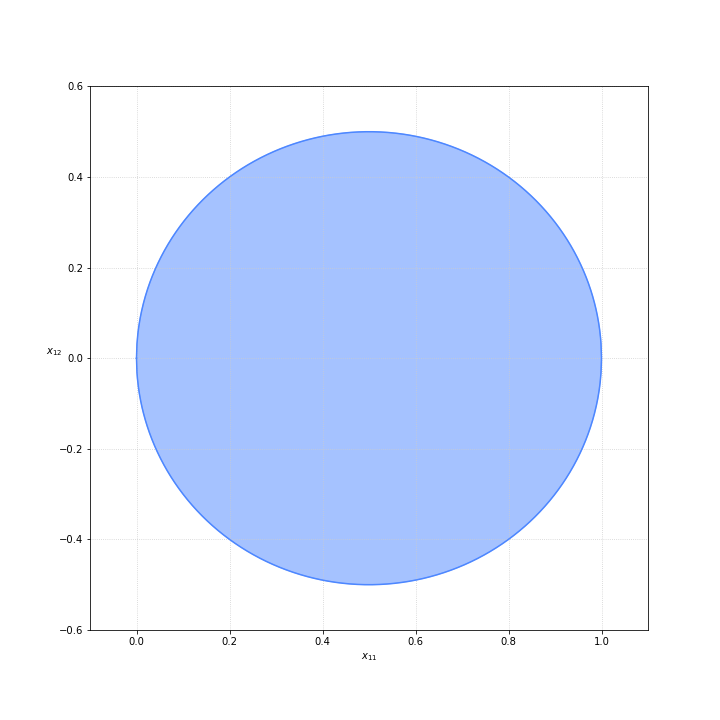
\includegraphics[width=0.5\textwidth]{img/ex3.png}   
    \caption{Přípustná množina řešení k úloze~\ref{eq:P3}.}
    \label{fig:ex3}
\end{figure}

\section{Dualita}

\subsubsection*{Duální úloha}

Podobně jako u lineárního programování použijeme Lagrangeovu dualitu k odvození duální úlohy k \ref{eq:SDP-P}. Lagrangeova funkce je ve tvaru
$$
    L(X, \lambda, Z) = \langle C, X \rangle - \sum_{i=1}^m \lambda_i \left( \langle A_i, X \rangle - b_i \right) - \langle Z, X \rangle.
$$

\noindent K ní duální funkce
$$
    d(\lambda, Z) = \inf_{X \in S^n} L(X, \lambda, Z) = 
    \begin{cases}
        \lambda^T b & \dots\ C - \sum_{i=1}^m \lambda_i A_i - Z = 0, \\
        -\infty     & \dots\ \text{jinak.}
    \end{cases}
$$

\noindent Duální funkci použijeme v duální úloze
\begin{equation}\tag{SDP-D}
    \sup\left\{ \lambda^Tb \mid C - \sum_{i=1}^m \lambda_i A_i \succeq 0 \right\},
    \label{eq:SDP-D}
\end{equation}
kde $\lambda = (\lambda_1, \dots, \lambda_m)$ je duální proměnná.

\noindent Dostali jsme duální úlohu~\ref{eq:SDP-D} k úloze~\ref{eq:SDP-P}.

\subsubsection*{Slabá dualita semidefinitního programování}

Vztah mezi primární a duální úlohou je stejně jako u lineárního programování takový, že řešení jedné úlohy lze použít jako odhad na úlohu druhou. Nechť $X$ je libovolné přípustné řešení primární úlohy a $y$ je libovolné přípustné řešení duální úlohy. Potom
\begin{equation}
    \langle C, X \rangle - b^T y =
    \langle C, X \rangle - \sum_{i=1}^m y_i \langle A_i, X \rangle =
    \left\langle C - \sum_{i=1}^m A_i y_i, X \right\rangle \geq 0.
    \label{eq:weak_duality_SDP}
\end{equation}
Za pozornost stojí poslední nerovnost, která plyne z toho, že skalární součin dvou pozitivně semidefinitních matic je nezáporný. Odvození je následující. Mějme dvě matice $S, T \succeq 0$. Matici $S$ můžeme napsat jako součet \uv{rank one} matic. Označme $r_S = \textbf{rank}\ S$, tj.
$$
    S = \sum_{i=1}^{r_S} S_i = \sum_{i=1}^{r_S} \lambda_i s_i s_i^T.
$$
Dále se podíváme na součin $T \cdot S_i$. Tedy pro $i = 1, \dots, r_S$ platí
$$
    T \cdot S_i = \lambda_i s_i^T T s_i \geq 0,
$$
kde nerovnost plyne z toho, že matice $T$ je pozitivně semidefinitní.

O nerovnosti~\ref{eq:weak_duality_SDP} se mluví jako o slabé dualitě semidefinitního programování.

\subsubsection*{Silná dualita semidefinitního programování}

\begin{vt2}[podmínka optimality]
    Nechť $X$ je přípustné řešení úlohy~\ref{eq:SDP-P} a $y$ je přípustné řešení úlohy~\ref{eq:SDP-D} taková, že splňují podmínku (komplementární skluzovosti)
    $$
        \left( C - \sum_{i=1}^m A_i y_i \right) X = 0.
    $$
    Potom $X$ je optimální řešení úlohy~\ref{eq:SDP-P} a $y$ je optimální řešení úlohy~\ref{eq:SDP-D}.
\end{vt2}

Obracená implikace sama o sobě neplatí, což znamená, že obecně dualitní rozdíl u semidefinitního programování není nulový. Musíme přidat podmínku kvalifikace omezení, kterou je například již zmíněná Slaterova podmínka. Ta je pro úlohu~\ref{eq:SDP-P} ve tvaru $X \succ 0$ a pro úlohu~\ref{eq:SDP-D} ve tvaru $C - \sum_i A_i y_i \succ 0$.

\begin{vt2}[silná dualita semidefinitního programování]
    Nechť úloha~\ref{eq:SDP-P} a úloha~\ref{eq:SDP-D} jsou striktně přípustné. Potom dualitní rozdíl jejich optimálních řešení je nulový.
\end{vt2}


\section{Vektorové programování}

Mějme $n$ vektorových proměnných $v_1, \dots, v_n$ v $\mathbb{R}^n$. \textbf{Vektorový program} je problém optimalizace lineární funkce skalárních součinů $\langle v_i, v_j \rangle$, vzhledem k lineárním omezením na tyto skalární součiny.

Nyní ukážeme, že vektorové programy jsou ekvivalentní semidefinitním programům. Nechť tedy $\mathcal{V}$ je vektorový program s vektorovými proměnnými $v_1, \dots, v_n$ v $\mathbb{R}^n$ a $\mathcal{S}$ je příslušný semidefinitní program s $n^2$ proměnnými $y_{ij}$, kde hodnota $y_{ij}$ odpovídá skalárnímu součinu $\langle v_i, v_j \rangle$. Matice $Y$ je navíc pozitivně semidefinitní. Potom platí následující věta.

\begin{vt2}
    Vektorový program $\mathcal{V}$ je ekvivalentní semidefinitnímu programu $\mathcal{S}$.
\end{vt2}

\begin{proof}
    TODO
\end{proof}


% \section*{BACKLOG}
% 
% Stopa matice $A \in R^{n \times n}$ je $\textbf{Tr}(A) = \sum_{i=1}^n A_{ii}$.
% 
% \begin{vt}
% $S, T$ jsou pozitivně definitní $\implies$ $S + T$ je pozitivně definitní
% \end{vt}
% 
% \begin{proof}
% $x^T (S+T) x = x^T S x + x^T T x > 0$
% \end{proof}
% 
% 
% \noindent Úlohy s racionálními daty nemusí mít racionální optimální řešení.
% \noindent příklad
% 
% \noindent Jen 3 kužely s vlastnostmi jako PSD cone. Zmrzlina, a ještě jeden.
% \noindent Vnitřek $S_+^n$ je $S_{++}^n$.
% 
% \noindent Fejérova věta


%spektraedr, formulace, dualita, semidefinitní kužel, duální kužel, ...
%vektorové programování a jeho ekvivalence, formulace úloh
\clearpage


% ------------------------- ČÁST: KOMBINATORICKÉ ÚLOHY ----------------------- %
\part{Kombinatorické úlohy}

\chapter{Shannonova kapacita}

Kapitola je zpracována z \cite{approximation-algorithms-and-semidefinite-programming} a citovaných článků. \uv{Zřejmá} tvrzení jsou více rozepsána.

\section{Formulace úlohy}

Představme si komunikační kanál, kterým posíláme zprávy. Tyto zprávy jsou složeny ze symbolů nějaké konečné abecedy. Vlivem šumu mohou být některé symboly druhou stranou špatně interpretovány a naším cílem je vybrat co největší množinu slov délky $k$ tak, aby žádná dvě odeslaná slova nebyla vlivem tohoto šumu zaměnitelná.

Problém si formalizujeme v řeči teorie grafů. Mějme neorientovaný graf $G = (V, E)$, kde množina vrcholů představuje symboly z konečné abecedy a dva vrcholy $x, y$ jsou spojeny hranou, pokud vrchol $x$ může být vlivem šumu zaměněn za $y$.

Maximální počet nezaměnitelných zpráv délky $1$ je roven $\alpha(G)$, kde $\alpha(G)$ značí velikost největší nezávislé množiny v grafu $G$. Pro popis delších zpráv definujeme \textbf{silný součin} $G \cdot H$ grafů $G$ a $H$ následovně
\begin{equation*}
    V(G \cdot H) = V(G) \times V(H),
\end{equation*}
\begin{equation*}
    \begin{split}
    E(G \cdot H) = &\left\{ (i,u)(j,v) \mid ij \in E(G) \wedge uv \in E(H) \right\} \cup \\
                   &\left\{ (i,u)(j,v) \mid ij \in E(G) \wedge u = v \right\} \cup \\
                   &\left\{ (i,u)(j,v) \mid i = j \wedge uv \in E(H) \right\}.
    \end{split}
\end{equation*}

\begin{pr}
Pro graf $P_4 = a-b-c-d-e$ je silný součin $P_4 \cdot P_4$ zobrazen na obrázku~\ref{fig:strong_product_P4_P4}, ze kterého je hezky vidět, že např. zpráva $cd$ (na obrázku červeně) může být zaměněna s $bc$, $bd$, $be$, $cc$, $ce$, $dc$, $dd$ a $de$ (na obrázku oranžově). Podobně pro další zprávy.
\end{pr}

\begin{figure}[h!]
    \centering
    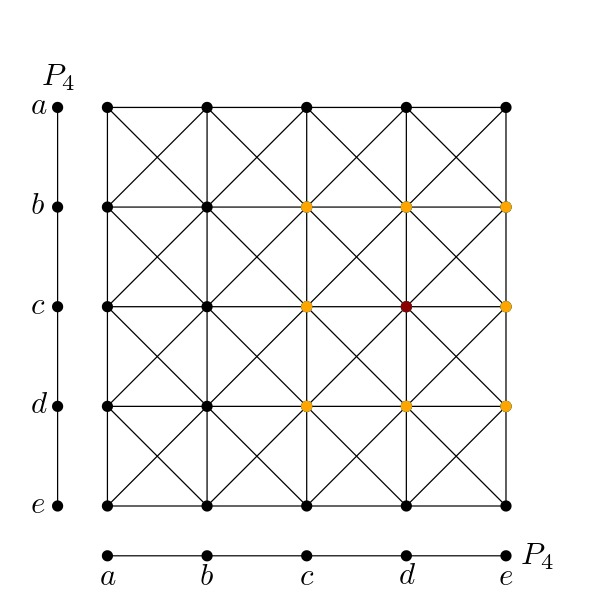
\includegraphics[width=0.5\textwidth]{img/strong_product_P4_P4.png}   
    \caption{$P_4 \cdot P_4$}
    \label{fig:strong_product_P4_P4}
\end{figure}

Pro jednoduchost budeme silný součin $k$ kopií grafu $G$ značit $G^k$. Tedy $\alpha(G^k)$ je maximální počet nezaměnitelných zpráv délky $k$. \textbf{Shannonova kapacita} grafu $G$ je definována jako
$$
    \Theta(G) = \sup \left\{ \alpha(G^k)^{1/k} \mid k = 1, 2, \dots \right\}.
$$

Neví se, zda pro libovolný graf $G$ existuje vůběc nějaký algoritmus, kterým bychom určili hodnotu $\Theta(G)$. Přesto je alespoň něco známo. Pro perfektní grafy Claude E. Shannon \textbf{[REF]} ukázal, že $\Theta(G) = \alpha(G)$. To také znamená, že pro perfektní grafy lze $\Theta(G)$ určit v polynomiálním čase. Dalším kdo se problémem zabýval byl László Lovász \textbf{[REF]}, který velmi hezkým způsobem ukázal, že kružnice délky $5$ má kapacitu $\sqrt{5}$. Na Lovászův postup se dále podíváme, protože vede k obecnému hornímu odhadu na $\Theta(G)$.

\section{$\Theta(C_5) = \sqrt{5}$}

Nejprve potřebujeme zavést několik pojmů. \textbf{Tenzorový součin} vektorů $u = \left(u_1, \dots, u_n \right)$ a $v = \left(v_1, \dots, v_m \right)$ je
$$
    u \circ v = \left( u_1 v_1, \dots, u_1 v_m, u_2 v_1, \dots, u_n v_m \right).
$$

Užitečné bude následující pozorování, které dává do souvislosti skalární a tenzorový součin.

\begin{pz}
    Nechť $x, u$ jsou vektory délky $n$ a $y, v$ jsou vektory délky $m$. Potom platí
    \begin{equation}
        \left( x \circ y \right)^T \left( u \circ v \right) = \left( x^T u \right) \left( y^T v \right).
        \label{eq:tensor_scalar_product}
    \end{equation}
\end{pz}

\begin{proof}
    Levá strana:
    \begin{equation*}
        \begin{split}
        & \left(x_1 y_1, x_1 y_2, \dots, x_1 y_m, \dots, x_n y_m \right)^T \left( u_1 v_1, u_1 v_2, \dots, u_1 v_m, \dots, u_n v_m \right) = \\
        & x_1 y_1 u_1 v_1 + x_1 y_2 u_1 v_2 + \dots + x_1 y_m u_1 v_m + \dots + x_m y_m u_n v_m
        \end{split}
    \end{equation*}
    Pravá strana:
    \begin{equation*}
        \begin{split}
            & \left( x_1 u_1 + \dots + x_n u_n \right) \cdot \left( y_1 v_1 + \dots + y_n v_m \right) = \\
            & x_1 y_1 u_1 v_1 + x_1 y_2 u_1 v_2 + \dots + x_1 y_m u_1 v_m + \dots + x_m y_m u_n v_m
        \end{split}
    \end{equation*}
\end{proof}

Mějme graf $G = (V,E)$, kde $V = \left\{ 1, \dots, n \right\}$. Systém $\left( v_1, \dots, v_n \right)$ jednotkových vektorů v Euklidovském prostoru takový, že
$$
    \forall ij \notin E \implies v_i \perp v_j
$$
nazýváme \textbf{ortonormální reprezentace} grafu $G$. Poznamenejme, že každý graf má nějakou ortonormální reprezentaci, např. $1 \mapsto e_1, \dots, n \mapsto e_n$.

\begin{lm}\textbf{[REF]}
    Nechť $\left( u_1, \dots, u_n \right)$ je ortonormální reprezentace grafu $G$ a $\left( v_1, \dots, v_m \right)$ je ortonormální reprezentace grafu $H$. Potom $u_i \circ v_j$ je ortonormální reprezentace grafu $G \cdot H$.
    \label{lemma:shannon}
\end{lm}

\begin{proof}
    Použijeme vztah \ref{eq:tensor_scalar_product}. $\left( u_i \circ v_j \right)^T \left( u_k \circ v_l \right) = \left( u_i^T u_k \right) \left( v_j^T v_l \right) = 0 \iff ik \notin E(G) \vee jl \notin E(H)$.
\end{proof}

\begin{figure}[h!]
    \centering
    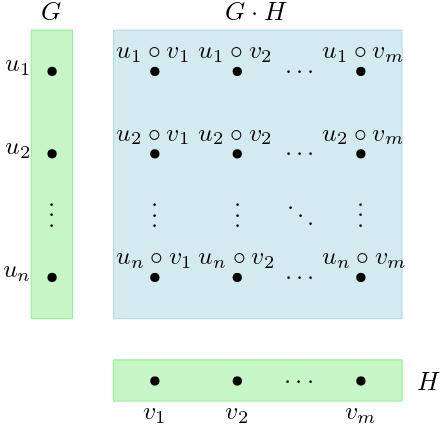
\includegraphics[width=0.5\textwidth]{img/shannon_lemma.png} 
    \caption{Lemma~\ref{lemma:shannon}}
\end{figure}

\noindent \textbf{Hodnotu} ortonormální reprezentace $\left(u_1, \dots, u_n \right)$ definujeme jako
$$
    \min_c \max_{i = 1, \dots, n} \frac{1}{\left( c^T u_i \right)^2}.
$$
Vektoru $c$, pro který nastává minimum říkáme \textbf{handle} dané ortonormální reprezentace.

Dále definujeme funkci $\vartheta(G)$ jako minimální hodnotu přes všechny ortonormální reprezentace grafu $G$. Ortonormální reprezentaci, pro kterou nastává minumum nazýváme \textbf{optimální}. Funkci $\vartheta(G)$ se říká \textbf{Lovászova theta funkce} a ona je právě již zmíněným horním odhadem na $\Theta(G)$. Podívejme se na některé její vlastnosti.

\begin{lm}\textbf{[REF]}
    $\vartheta(G \cdot H) \leq \vartheta(G) \vartheta(H)$
\end{lm}

\begin{proof}
    Nechť $\left( u_1, \dots, u_n \right)$ je optimální ortonormální reprezentace grafu $G$ s handle $c$ a $\left( v_1, \dots, v_m \right)$ je optimální ortonormální reprezentace grafu $H$ s handle $d$. Pak $c \circ d$ je jednotkový vektor a platí
    $$
        \vartheta(G \cdot H) \leq \max_{i,j} \frac{1}{\left( \left( c \circ d \right)^T \left( u_i \circ v_j \right) \right)^2} = \max_i \frac{1}{\left( c^T u_i \right)^2} \cdot \max_j \frac{1}{\left( d^T v_j \right)^2} = \vartheta(G)\vartheta(H).
    $$
\end{proof}

\begin{lm}\textbf{[REF]}
    $\alpha(G) \leq \vartheta(G)$
\end{lm}

\begin{proof}
    Mějme maximální nezávislou množinu $I \subseteq V(G)$ v grafu $G$ a optimální ortonormální reprezentaci $\mathcal{U} = \left( u_1, \dots, u_n \right)$ grafu $G$ s handle $c$. Platí
    $$
        \forall i,j \in I:\ i \neq j \implies u_i \bot u_j.
    $$
    Máme tedy systém ortonormálních vektorů $\left\{ u_i \in \mathcal{U} \mid i \in I \right\}$ v $\mathbb{R}^n$. Ten rozšíříme na ortonormální bázi $\mathcal{B}$. Potom $i$-tá souřadnice vektoru $c$ v bázi $\mathcal{B}$ je $c^T u_i$. Tedy
    $$
        1 = \| c \|^2 = \sum_{i=1}^n \left( c^T u_i \right)^2.
    $$
    Dále vynecháme přidáné vektory do ortonormální báze $\mathcal{B}$
    $$
        \sum_{i=1}^n \left( c^T u_i \right)^2 \geq \sum_{i \in I} \left( c^T u_i \right)^2.
    $$
    Poslední výraz přepíšeme
    $$
        \sum_{i \in I} \left( c^T u_i \right)^2 \geq |I| \cdot \min_{i \in I}\left( c^T u_i \right)^2 = \alpha(G) \cdot \min_{i \in I}\left( c^T u_i \right)^2.
    $$
    Předchozí výrazy dáme dohromady
    $$
        1 \geq \alpha(G) \cdot \min_{i \in I}\left( c^T u_i \right)^2,
    $$
    a dostáváme
    $$
        \alpha(G) \leq \frac{1}{\min_{i \in I}\left( c^T u_i \right)^2} = \max_{i \in I} \frac{1}{\left( c^T u_i \right)^2} \leq \max_{i \in V(G)} \frac{1}{\left( c^T u_i \right)^2} = \vartheta(G).
    $$
\end{proof}

\begin{lm}\textbf{[REF]}
    $\Theta(G) \leq \vartheta(G)$
\end{lm}

\begin{proof}
    Pro každé $k$ platí, že
    $$
        \alpha(G^k) \leq \vartheta(G^k) \leq \vartheta(G)^k.
    $$
    Odtud
    $$
        \sqrt[k]{\alpha(G^k)} \leq \vartheta(G),
    $$
    a limitním přechodem dostáváme požadovanou nerovnost
    $$
        \Theta(G) = \lim_{k \to \infty} \sqrt[k]{\alpha(G^k)} \leq \vartheta(G).
    $$
\end{proof}

\begin{vt}\textbf{[REF]}
    $\Theta(C_5) = \sqrt{5}$
\end{vt}

\begin{proof}
    Ukážeme konstrukci ortonormální reprezentace grafu $C_5$, ze které dostaneme horní odhad na $\Theta(C_5)$. Nechť $V(C_5) = \left\{ v_1, \dots, v_5 \right\}$ a $E(C_5) = \left\{ v_1v_2, v_2v_3, v_3v_4, v_4v_5, v_1v_5 \right\}$. Mějme vektory $\bar{u}_i$ ve tvaru
    $$
        \bar{u}_i = \left( \cos\frac{2 \pi i}{5}, \sin \frac{2 \pi i}{5}, z \right), i = 1, \dots, 5.
    $$
    Každý vektor $\bar{u}_i$ je svázán s vrcholem $v_i$. Chceme, aby dva vektory, které jsou příslušné nesousedním vrcholům, byly ortogonální. Tedy například $\langle \bar{u}_2, \bar{u}_5 \rangle = 0$. Dosadíme
    $$
        \left\langle \bar{u}_2, \bar{u}_5 \right\rangle = 
        \left\langle ( \cos\frac{4\pi}{5}, \sin\frac{4\pi}{5}, z ), \left( 1, 0, z \right) \right\rangle =
        \cos\frac{4\pi}{5} + z^2 = 0.
    $$
    Dostáváme tedy
    $$
        z = \sqrt{-\cos\frac{4\pi}{5}}.
    $$
    Definujeme ortonormální reprezentaci $\mathcal{U}$ grafu $C_5$ (projekce do první a druhé souřadnice, viz Obrázek~\ref{fig:umbrella_projection}) tak, že
    $$
        u_i = \frac{\bar{u}}{\| \bar{u} \|}, i = 1, \dots, 5,
    $$
    s handle $c = \left( 0, 0, 1 \right)$.
    Dostáváme
    $$
        \vartheta(C_5) \leq \vartheta(\mathcal{U}) = \max_{i = 1, \dots, 5} \frac{1}{(c^T u_i)^2} = \frac{1}{( c^T u_5)^2} = \frac{1 - \cos\frac{4\pi}{5}}{-\cos\frac{4\pi}{5}}.
    $$
    Do posledního výrazu dosadíme známou hodnotu pro $\cos 36^{\circ}$.
    $$
        \frac{1 - \cos\frac{4\pi}{5}}{-\cos\frac{4\pi}{5}} = \frac{1 + \frac{1 + \sqrt{5}}{4}}{\frac{1 + \sqrt{5}}{4}} = \frac{5 + \sqrt{5}}{1 + \sqrt{5}} = \sqrt{5}.
    $$
    Dostáváme
    $$
        \vartheta(C_5) \leq \sqrt{5}.
    $$
    Této ortonormální reprezentaci se říká \textbf{Lovászův deštník}, viz Obrázek~\ref{fig:umbrella}. Druhou nerovnost $\vartheta(C_5) \geq \sqrt{5}$ dostaneme snadno. Sice $\alpha(C_5) = 2$, ale $\alpha(C_5^2) = 5$. Z čehož plyne druhá nerovnost.
\end{proof}

\begin{figure}[h!]
    \centering
    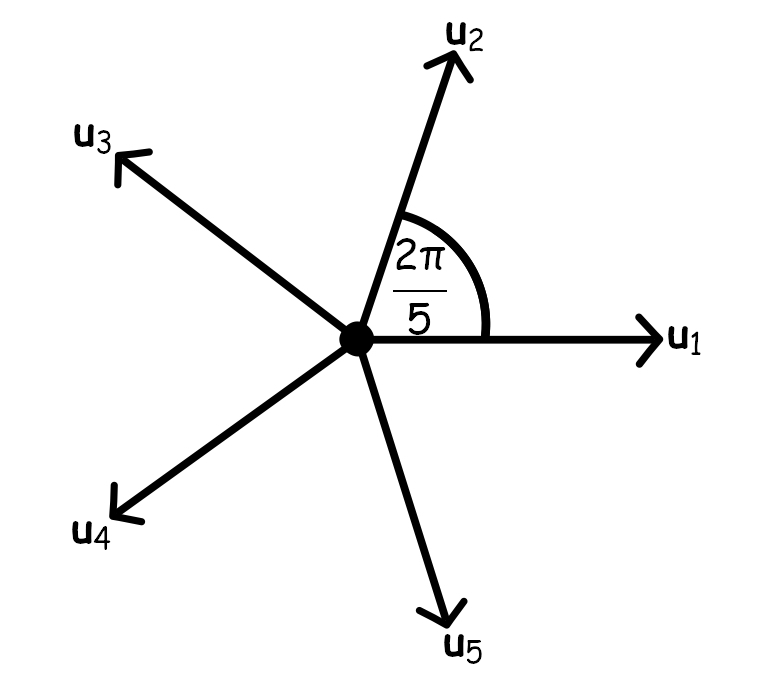
\includegraphics[width=0.5\textwidth]{img/umbrella_projection.png} 
    \caption{Projekce $u_i$ do první a druhé souřadnice.}
    \label{fig:umbrella_projection}
\end{figure}

\begin{figure}[h!]
    \centering
    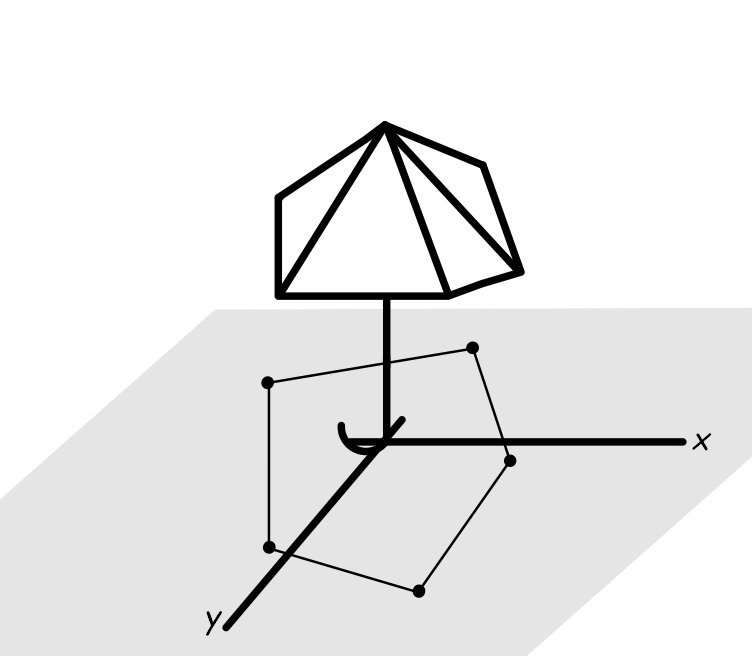
\includegraphics[width=0.5\textwidth]{img/umbrella.png} 
    \caption{Lovászův deštník.}
    \label{fig:umbrella}
\end{figure}


\section{Semidefinitní programy pro $\vartheta(G)$}

\subsection*{Program pro $1/\sqrt{\vartheta}$}

První formulací je semidefinitní program (\textbf{[REF]}), jehož řešením je hodnota $\frac{1}{\sqrt{\vartheta}}$. Mějme graf $G = (V,E)$. Hodnota $\vartheta(G)$ je z definice
$$
    \vartheta(G) = \min_\mathcal{U} \vartheta(\mathcal{U}) = \min_\mathcal{U} \min_{\|c\|=1} \max_{i \in V(G)} \frac{1}{\left( c^T u_i \right)^2},
$$
kde $\mathcal{U}$ probíhá přes všechny ortonormální reprezentace grafu $G$. Pokud se stane, že $c^T u_i \leq 0$, potom místo $u_i$ budeme dále uvažovat vektor $-u_i$. Můžeme tedy předpokládat, že $\forall i \in V(G):\ c^T u_i \geq 0$. Potom hodnotu $1/\sqrt{\vartheta(G)}$ můžeme vyjádřit jako
$$
    \frac{1}{\sqrt{\vartheta(G)}} = \max_\mathcal{U} \frac{1}{\sqrt{\vartheta(\mathcal{U})}} = \max_\mathcal{U} \max_{\|c\|=1} \min_{i \in V(G)} c^T u_i.
$$
Z čehož dostaneme následující vektorový program
\begin{equation}\tag{VP1}
    \begin{split}
        &\max t \\
        &\forall ij \in E(\bar{G}):\ \langle u_i, u_j \rangle = 0 \\
        &\forall i \in V(G):\ \langle c, u_i \rangle \geq t \\
        &\forall i \in V(G):\ \| u_i \| = 1 \\
        &\| c \| = 1.
    \end{split}
    \label{eq:VP1}
\end{equation}

Z vektorového programu~\ref{eq:VP1} dále odvodíme semidefinitní program. Budeme uvažovat matici
$$
    X =
    \begin{bmatrix}
        \horzbar & c^T    & \horzbar \\
        \horzbar & u_1^T  & \horzbar \\
                 & \vdots &          \\
        \horzbar & u_n^T  & \horzbar
    \end{bmatrix}
    \begin{bmatrix}
        \vertbar & \vertbar &       & \vertbar \\
        c        & u_1      & \dots & u_n      \\
        \vertbar & \vertbar &       & \vertbar \\
    \end{bmatrix},
$$
která je samozřejme pozitivně semidefinitní.
Podmínkám $\forall i \in V(G):\ \| u_i \| = 1$ a $\|c\|=1$ odpovídá podmínka $x_{ii} = 1$ pro $i = 0, 1, \dots, n$ (pro teď budeme indexovat matici $X$ od $0$). Podmínku $\forall ij \in E(\bar{G}):\ \langle u_i, u_j \rangle = 0$ přepíšeme na
$$
    \forall ij \in E(\bar{G}):\ x_{ij} = 0.
$$
A konečně poslední podmínku $\forall i \in V(G):\ \langle c, u_i \rangle \geq t$ přepíšeme takto
$$
    \forall i \in V(G):\ x_{0i} \geq t.
$$
Dostáváme tedy semidefinitní program
\begin{equation}\tag{SDP1}
    \begin{split}
        &\max t \\
        &x_{ii} = 1, i = 0, 1, \dots, n \\
        &\forall ij \in E(\bar{G}):\ x_{ij} = 0 \\
        &\forall i \in V(G):\ x_{0i}  \geq t \\
        &X \succeq 0.
    \end{split}
    \label{eq:SDP1}
\end{equation}


\subsection*{Program pro $\vartheta$}

V původním článku od L.~Lovásze \textbf{[REF]} je další semidefinitní program, jehož řešením je přímo hodnota $\vartheta(G)$.

\begin{equation}\tag{SDP2}
    \begin{split}
        &\max \langle X, J \rangle \\
        &\forall ij \in E(G):\ x_{ij} = 0 \\
        &\textbf{Tr}\ X = 1 \\
        &X \succeq 0,
    \end{split}
    \label{eq:SDP2}
\end{equation}
kde $J$ je matice samých jedniček.

\section{$\vartheta$ a související grafové parametry}

Začneme tzv. Sendvičovou větou a dále zaměříme na grafy $C_5$, $C_7$, Petersenův graf, $K_5$ a $S_5$.

\begin{vt}\textbf{[REF]}
    Mějme graf $G$ a jeho doplněk $\bar{G}$. Potom
    $$
        \alpha(G) \leq \vartheta(G) \leq \chi(\bar{G}).
    $$
\end{vt}

\subsection*{$\alpha(G)$ pro vybrané grafy}
Je zřejmé, že pro $\alpha(C_5) = 2$, $\alpha(C_7) = 3$, $\alpha(K_5) = 1$ a $\alpha(S_5) = 5$. Na obrázku~\ref{fig:alpha_petersen} je, pro Petersenův graf, nezávislá množina velikosti $4$. Probírkou všech možností zjistíme, že větší nezávislou množinu se nám najít nepodaří.

\begin{figure}[h!]
    \centering
    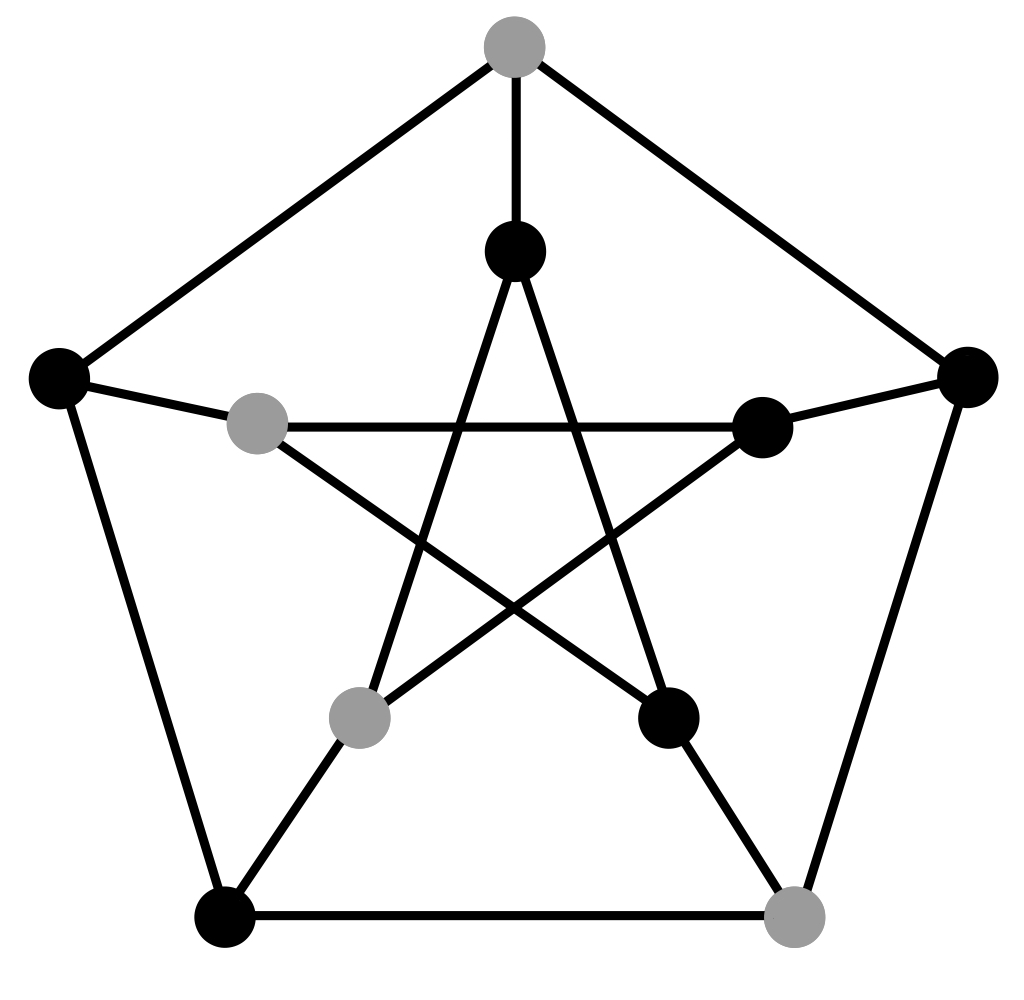
\includegraphics[width=0.5\textwidth]{img/alpha_petersen.jpeg}   
    \caption{Největší nezávislá množina v $GP_{5,2}$.}
    \label{fig:alpha_petersen}
\end{figure}

\subsection*{$\chi(\bar{G})$ pro vybrané grafy}

Doplněk $C_5$ je opět $C_5$ a lichá kružnice má chromatické číslo $3$. $K_5$ má jako svůj doplněk diskrétní graf, který má chromatické číslo $1$. U hvězdy $S_5$ dostaneme jako doplněk graf s šesti vrcholy, kde pět z nich tvoří úplný graf a jeden vrchol nemá žádného souseda. Takový graf má chromatické číslo $5$. Pro Petersenův graf je jeho doplněk $T_5$, který má $\chi(T_5) = 5$ ($T_5$ viz Obrázek~\ref{fig:complement_petersen}). Nakonec doplněk k $C_7$ je na obrázku~\ref{fig:complement_c7} a opět probírkou všech možností zjistíme, že chromatické číslo je $4$.

\begin{figure}[h!]
    \centering
    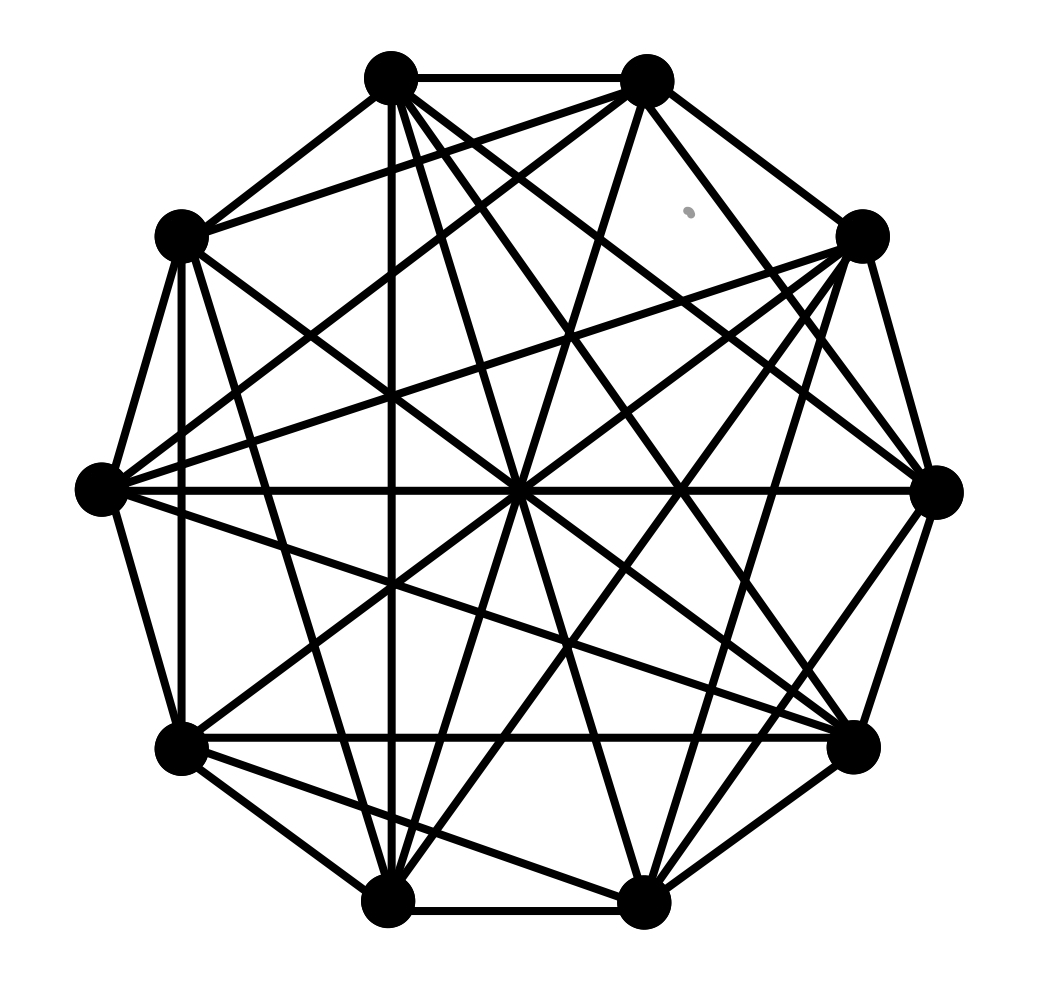
\includegraphics[width=0.5\textwidth]{img/complement_petersen.jpeg}   
    \caption{Triangular graf $T_5$.}
    \label{fig:complement_petersen}
\end{figure}

\begin{figure}[h!]
    \centering
    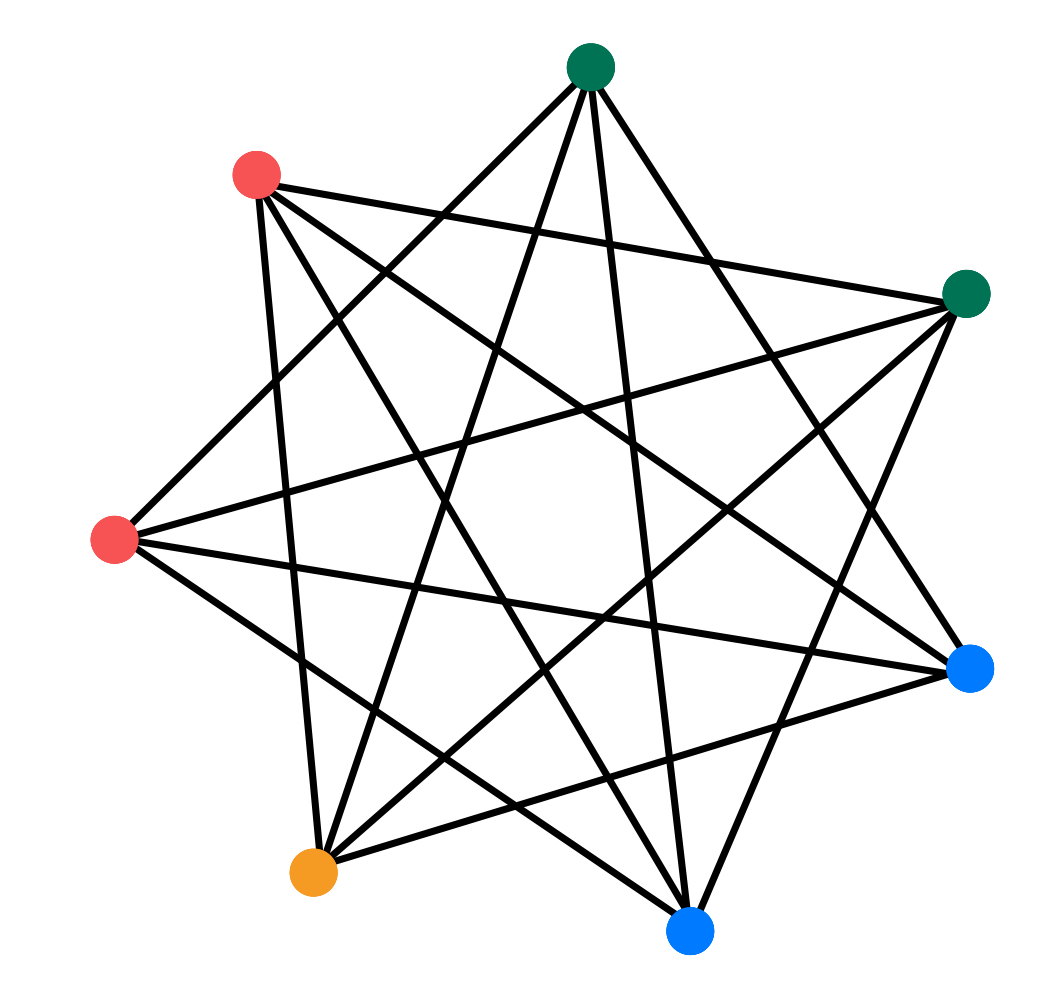
\includegraphics[width=0.5\textwidth]{img/complement_c7.jpeg}   
    \caption{Obarvení $\bar{C_7}$.}
    \label{fig:complement_c7}
\end{figure}

\subsection*{$\vartheta(G)$ pro vybrané grafy}

Dříve jsme ukázali, že $\vartheta(C_5) = \sqrt{5} \approx 2.2361$. Navíc pro liché $n$ \textbf{[REF]} platí, že
\begin{equation}
    \vartheta(C_n) = \frac{n \cdot \cos(\frac{\pi}{n})}{1 + \cos(\frac{\pi}{n})}.
    \label{eq:cycle_theta}
\end{equation}
Dostáváme tedy, že $\vartheta({C_7}) \approx 3.3177$. Zbylé hodnoty plynou ze sendivičové věty. V tabulce~\ref{tab:sandwitch} jsou shrnuty všechny zmíněné hodnoty.

\begin{table}[h!]
    \centering
    \begin{tabular}{ c | c c c }
        $G$        & $\alpha(G)$ & $\vartheta(G)$ & $\chi(\bar{G})$ \\
        \hline
        $C_5$      & $2$         & $2.2361$       & $3$ \\  
        $C_7$      & $3$         & $3.3177$       & $4$ \\
        $GP_{5,2}$ & $4$         & $4$            & $5$ \\
        $K_5$      & $1$         & $1$            & $1$ \\
        $S_5$      & $5$         & $5$            & $5$
    \end{tabular}
    \caption{$\alpha(G)$, $\vartheta(G)$, $\chi(\bar{G})$ pro vybrané grafy.}
    \label{tab:sandwitch}
\end{table}

\subsection*{Co víme o $\Theta(G)$}

Shannonova kapacita je známá jen pro několik málo grafů. V \textbf{[REF]} Shannon dal dolní odhad na $\Theta(C_5)$ a až za 23 let Lovász ukázal pomocí konstrukce, kterou jsme si ukázali výše, že $\Theta(C_5) = \sqrt{5}$. Ve stejném článku \textbf{[REF]} je důkaz, že kapacita Petersenova grafu $GP_{5,2}$ je $4$. Triviální případy $S_5$ a $K_5$ dostaneme ze sendvičové věty, tj. $\Theta(S_5) = 5$ a $\Theta(K_5) = 1$. Naopak pro $C_7$ hodnotu $\Theta$ neznáme. Máme dolní odhad $\alpha(C_7) = 3$ a horní odhad $\vartheta(C_7) \approx 3.3177$. Lepší dolní odhad, než dává $\alpha(C_7)$, ukázali Polak a Schriever \textbf{[REF]} tak, že pomocí počítače našli nezávislou množinu v grafu $C_7^5$ velikosti $367$. Z čehož dostaneme dolní odhad $\sqrt[5]{367} \approx 3.2579$. Hodnota $\Theta(C_7)$ je tedy někde mezi
$$
    3.2578 < \Theta(C_7) \leq 3.3177.
$$

Poznamenejme, že vylepšit dolní odhad na $\Theta(C_7)$ je výpočetně náročná úloha. Už pro $C_7^4$ se pomocí formulace
\begin{equation*}
    \begin{split}
        &\max \sum_{i=1}^n x_i \\
        &\forall ij \in E:\ x_i + x_j \leq 1 \\
        &\forall i \in V:\ x_i \in \left\{ 0, 1 \right\}
    \end{split}
\end{equation*}
nenajde užitečná nezávislá množina, která by měla velikost alespoň $108$ \textbf{[REF-Vesel-Žertovnik]}. K výpočtu byl použit framework \textbf{Gurobi} a program po $7$ měsících našel pouze nezávislou množinu velikosti $102$, která dává dolní odhad $\sqrt[4]{102} \approx 3.1779$.


\section{Experimenty}

Porovnáme formulace \ref{eq:SDP1} a \ref{eq:SDP2}, které byly naimplementovány ve frameworku \textbf{Mosek}, na lichých kružnicích s přesnou hodnotou a dále určíme hodnoty $\vartheta$ pro náhodné grafy řádu $30$.

\subsection{Liché kružnice}

V tabulce~\ref{tab:cycles_theta} jsou napočítané hodnoty $\vartheta$ funkce pro liché kružnice pomocí formulací \ref{eq:SDP1} a \ref{eq:SDP2}. Tučně jsou zvýrazněny číslice, které se shodují s přesnou hodnotou určenou ze vztahu~\ref{eq:cycle_theta}.

\begin{table}[h!]
    \begin{center}
        \begin{tabular}{ c | c c c }
        $m$     & $\vartheta(C_n)$ & \ref{eq:SDP1}          & \ref{eq:SDP2} \\
        \hline
        $5$     & $2.236067977$    & $\mathbf{2.23606}8103$ & $\mathbf{2.23606797}8$ \\
        $7$     & $3.317667207$    & $\mathbf{3.317667}960$ & $\mathbf{3.317667207}$ \\
        $9$     & $4.360089581$    & $\mathbf{4.3600895}96$ & $\mathbf{4.360089}606$ \\
        $11$    & $5.386302911$    & $\mathbf{5.3863029}51$ & $\mathbf{5.38630291}4$ \\
        $13$    & $6.404168562$    & $\mathbf{6.404168}697$ & $\mathbf{6.404168562}$ \\
        $15$    & $7.417148247$    & $\mathbf{7.41714}9582$ & $\mathbf{7.417148247}$ \\
        $\dots$ & $\dots$          & $\dots$                & $\dots$ \\
        $121$   & $110.494417456$  & nedoběhlo              & $\mathbf{110.494417456}$ \\
        \end{tabular}
    \end{center}
    \caption{Porovnání implementací $\vartheta$ funkce na lichých kružnicích.}
    \label{tab:cycles_theta}
\end{table}

Jednodušší model \ref{eq:SDP2} dává přesnější výsledky a je schopen upočítat i větší úlohy. Nepřesnosti jsou dány tím, že solver v modelu \ref{eq:SDP1} má mnohem více omezení a dvě proměnné $X \succeq 0$, $t \geq 0$. Největší problém představuje omezení
$$
    \forall i \in V(G):\ x_{0i} \geq t.
$$
V implementaci se totiž od sebe odečítají dvě proměnné a to v tomto frameworku není doporučovaná operace.
 

\subsection{Náhodné grafy řádu $30$}

U větších grafů s nepravidelnou strukturou se rozdíly prohlubují a je vidět, že ani pro úplný graf, který je v tabulce~\ref{tab:random_theta} uveden na posledním řádku, není hodnota u \ref{eq:SDP1} přesná.

\begin{table}[h!]
    \begin{center}
        \begin{tabular}{ c | c c }
        $m$    & \ref{eq:SDP1}  &  \ref{eq:SDP2}  \\
        \hline
        $0$    & $30.000000007$ &  $30.0$         \\
        $43$   & $16.000005889$ &  $17.690577212$ \\
        $87$   & $11.151050632$ &  $14.385152039$ \\
        $130$  & $9.0000004168$ &  $11.557666814$ \\
        $174$  & $7.0892127153$ &  $9.9856302253$ \\
        $217$  & $6.1569911550$ &  $9.5632864871$ \\
        $261$  & $5.0000131024$ &  $7.6828991181$ \\
        $304$  & $4.0323146793$ &  $6.8219576402$ \\
        $348$  & $3.2171989901$ &  $5.1733914919$ \\
        $391$  & $3.0000021103$ &  $4.0513834517$ \\
        $435$  & $1.0000007203$ &  $1.0$          \\
        \end{tabular}
    \end{center}
    \caption{Výsledky implementací $\vartheta$ funkce na náhodných grafech řádu $30$ s daným počtem hran.}
    \label{tab:random_theta}
\end{table}



\clearpage

\chapter{Problém maximálníhu řezu}

\section{Formulace úloh}

Mějme neorientovaný graf $G = (V, E)$ s nezáporným ohodnocením hran $w$. Cílem je rozložit množinu vrcholů $V$ na nejvýše $k \geq 2$ disjunktních množin $V_1, \dots, V_k$ tak, aby součet vah hran vedoucí mezi různými množinami byl maximální. Pokud $k = 2$ hovoříme o úloze \textbf{MAX CUT} a pro $k \geq 3$ o úloze \textbf{MAX $k$-CUT}. Máme-li navíc předepsané maximální počty vrcholů v jednotlivách množinách, tj.
$$
    |V_1| \leq s_1, \dots, |V_k| \leq s_k,
$$
kde $|V| = n \leq \sum_i s_i$, jedná se o kapacitní MAX $k$-CUT úlohu, kterou budeme značit \textbf{CMAX $k$-CUT}. 

\section{Úloha MAX CUT}

Nejprve se podíváme na aproximační algoritmus z článku \textbf{[REF]} pro úlohu MAX CUT.

\subsection{Striktní kvadratický program pro MAX CUT}

\textbf{Kvadratický program} je problém optimalizace kvadratické funkce celočíselných proměnných, vzhledem ke kvadratickým omezením těchto proměnných. Je-li navíc každý monom (jednočlen) cenové funkce i daných omezení stupně $0$ nebo $2$, potom mluvíme o \textbf{striktním kvadratickém programu}.

Pomocí striktního kvadratického programu můžeme formulovat úlohu MAX CUT. Postup je následující. Nechť $y_i \in \left\{ 1, -1 \right\}$ je proměnná příslušná vrcholu $i$. Množiny $S$ a $\bar{S}$ definujeme tak, že
$$
    S = \left\{ i \in V \mid y_i = 1 \right\} \text{ a } \bar{S} = \left\{ i \in V \mid y_i = -1 \right\}.
$$
Pokud $i \in S$ a $j \in \bar{S}$, potom je součin $y_i y_j = -1$ a chceme, aby tato hrana přispívala hodnotou $w_{ij}$ k cenové funkci. Ve zbylých dvou možnostech je $y_i y_j = 1$ a chceme, aby se hodnota cenové funce nezměnila. Dostáváme následující striktní kvadratický program.

\begin{equation}\tag{SQ-MAX-CUT}
    \begin{split}
        OPT = &\max \frac{1}{2} \sum_{1 \leq i < j \leq n} w_{ij} (1 - y_i y_j) \\
        &\forall i \in V:\ y_i^2 = 1, \\
        &\forall i \in V:\ y_i \in \mathbb{Z}.
    \end{split}
    \label{eq:SQ-MAX-CUT}
\end{equation}


\subsection{Vektorový program pro MAX CUT}

Poznamenejme jen, že úloha celočíselného programování je NP-těžká. Proto se dále budeme zabývat relaxací úlohy~\ref{eq:SQ-MAX-CUT}, což znamená, že upustíme od podmínek celočíselnosti a původní úlohu aproximujeme vektorovým programem. Modifikujeme tedy program~\ref{eq:SQ-MAX-CUT} tak, že každý součin $y_i y_j$ nahradíme skalárním součinem vektorů $\langle v_i, v_j \rangle$ v $\mathbb{R}^n$. Dostáváme následující vektorový program.

\begin{equation}\tag{V-MAX-CUT}
    \begin{split}
        RELAX = &\max \frac{1}{2} \sum_{1 \leq i < j \leq n} w_{ij} (1 - \langle v_i, v_j \rangle) \\
        &\forall i \in V:\ \langle v_i, v_i \rangle = 1, \\
        &\forall i \in V:\ v_i \in \mathbb{R}^n.
    \end{split}
    \label{eq:V-MAX-CUT}
\end{equation}


\subsection{Semidefinitní program pro MAX CUT}

Vektorový program~\ref{eq:V-MAX-CUT} je ekvivalentní s příslušným semidefinitním programem (viz věta~\textbf{[REF]}). Nechť $W$ je vážená matice sousednosti grafu $G$ a $w_{ij}$ je váha hrany $ij$, kde $i < j$. Matice $J$ je matice $n \times n$ samých jedniček.

\begin{equation}\tag{SDP-MAX-CUT}
    \begin{split}
        RELAX = &\max \frac{1}{4} \langle W, J - Y \rangle \\
        &\forall i \in V:\ y_{ii} = 1, \\
        &Y \succeq 0.
    \end{split}
    \label{eq:SDP-MAX-CUT}
\end{equation}

\subsection{Aproximační algoritmus}

Vyřešením programu \ref{eq:SDP-MAX-CUT} dostaneme optimální řešení $Y^*$. Matice je samozřejmě pozitivně semidefinitní. Provedeme rozklad
$$
    Y^* = LL^T,
$$
kde řádky matice $L$ jsou optimální řešení vektorového programu \ref{eq:V-MAX-CUT}. Označme $i$-tý řádek matice $L$ jako $a_i$. Dále budeme chtít nějakým způsobem separovat vektory, které jsou od sebe \uv{daleko} a shlukovat ty, které jsou \uv{blízko}.

Označme $\Theta_{ij}$ úhel, který svírají vektory $a_i$ a $a_j$. Z podmínky
$$
    \forall i \in V:\ \langle v_i, v_i \rangle = 1
$$
dostáváme, že $\langle a_i, a_j \rangle = \cos \Theta_{ij}$ a příspěvěk těchto vektorů k optimálnímu řešení je
$$
    \frac{w_{ij}}{2} (1 - \cos \Theta_{ij}).
$$
Tedy čím \uv{blíž} je úhel $\Theta_{ij}$ hodnotě $\pi$, tím větší příspěvěk mají tyto vektory k hodnotě optimálního řešení. Algoritmus je následující.

\begin{alg}[MAX-CUT]$ $
    \begin{enumerate}
        \item Najdi řešení $a_1, \dots, a_n$ programu~\ref{eq:V-MAX-CUT}.
        \item Zvol náhodně vektor $r$ na jednotkové sféře $S_{n-1}$.
        \item $S = \left\{ i \in V \mid \langle a_i, r \rangle \geq 0 \right\}$.
    \end{enumerate}
    \label{alg:max-cut}
\end{alg}

Dále se budeme snažit objasnit kroky \textbf{1} a \textbf{2} v algoritmu~\ref{alg:max-cut}.

\begin{lm}
    Nechť $X_{ij}$ je jev takový, že vrcholy $i$ a $j$ jsou od sebe separovány, tj. jsou v různých množinách. Potom
    $$
        P\left[ X_{ij} \right] = \frac{\Theta_{ij}}{\pi}.
    $$
    \label{lemma:sep}
\end{lm}

\begin{proof}
    Vektory $a_i, a_j$ generují rovinu. Uvažme projekci náhodného vektoru $r$ na jednotkové sféře $S_{n-1}$ do této roviny. Potom vrcholy $i$ a $j$ jsou separovány, jestliže
    $$
        \langle a_i, a_j \rangle = \langle r, a_i \rangle + \langle r, a_j \rangle
    $$
    \begin{center}
        nebo
    \end{center}
    $$
        \langle a_i, a_j \rangle = \langle -r, a_i \rangle + \langle -r, a_j \rangle.
    $$
    Předchozí podmínku separace vrcholů ilustruje obrázek~\ref{fig:lemma_plane}.
\end{proof}

\begin{figure}[h!]
    \centering
    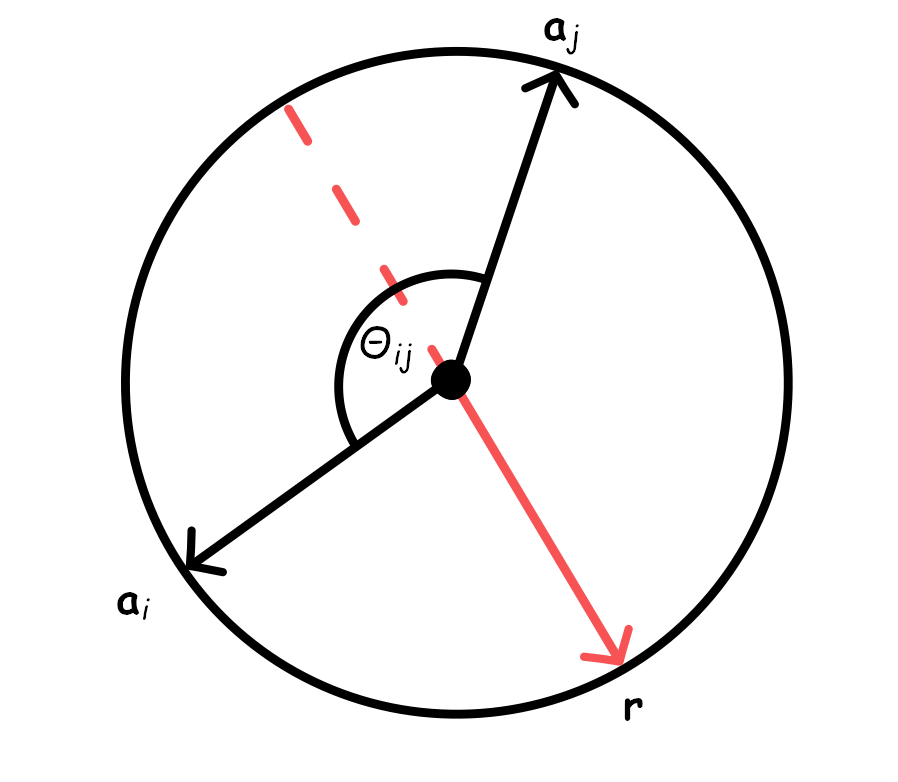
\includegraphics[width=0.5\textwidth]{img/lemma_plane.png}   
    \caption{Separace vrcholů $i$, $j$ náhodným vektorem $r$.}
    \label{fig:lemma_plane}
\end{figure}

\begin{lm}[KNUTH 2, 135]
    Nechť $x = (x_1, \dots, x_n)$ je vektor, jehož prvky jsou zvoleny nezávisle z normálního normovaného rozdělení $\mathcal{N}(0,1)$. Potom $r = \frac{x}{\| x \|}$ je náhodný vektor, který leží na jednotkové sféře $S_{n-1}$.
    \label{lemma:random-vector-on-sphere}
\end{lm}

Lemma~\ref{lemma:random-vector-on-sphere} nám dává postup, kterým provedeme bod \textbf{2} v algoritmu~\ref{alg:max-cut}. Nyní ukážeme, jak \uv{dobrou} aproximaci algoritmem~\ref{alg:max-cut} dostaneme. Označme
$$
    \alpha = \min_{0 \leq \Theta \leq \pi} \frac{2 \Theta}{\pi (1 - \cos \Theta)}.
$$
Snadno se ukáže, použitím derivace, že $\alpha \approx 0.87856$.

\begin{lm}
    Nechť $Y$ je náhodná veličina, která označuje součet vah hran, které vedou z $S$ do $\bar{S}$, nalezeny algoritmem~\ref{alg:max-cut}. Potom
    $$
        E\left[ Y \right] \geq \alpha \cdot RELAX.
    $$
\end{lm}

\begin{proof}
    Z definice čísla $\alpha$, pro $0 \leq \Theta \leq \pi$, dostáváme
    \begin{equation}
        \frac{\Theta}{\pi} = \frac{2 \Theta}{\pi (1 - \cos \Theta)} \cdot \frac{1 - \cos \Theta}{2} \geq \frac{\alpha}{2} (1 - \cos \Theta).
        \label{eq:proof_1}
    \end{equation}
    Použitím lemmatu~\ref{lemma:sep} a nerovnosti~\ref{eq:proof_1} dostáváme
    \begin{equation*}
        \begin{split}
            E\left[ Y \right] &= \sum w_{ij} P\left[ X_{ij} \right] \\
                              &= \sum w_{ij} \frac{\Theta_{ij}}{\pi} \\
                              &\geq \frac{\alpha}{2} \sum w_{ij} (1 - \cos \Theta_{ij}) \\
                              &= \alpha \cdot RELAX.
        \end{split}
    \end{equation*}
\end{proof}

\noindent Poznamenejme, že samozřejmě platí
\begin{equation}
    OPT \geq E\left[ Y \right] \geq \alpha \cdot RELAX.
    \label{eq:int-gap}
\end{equation}

\noindent \textbf{Mezeru celočíselnosti} relaxace (pro maximalizační problém) definujeme jako
$$
    \inf_{I} \frac{OPT(I)}{RELAX(I)},
$$
kde infimum probíhá přes všechny instance $I$ daného programu (pro minimalizační problém by se čitatel a jmenovat prohodily). Ze vztahu~\ref{eq:int-gap} dostáváme, že mezera celočíselnosti relaxace~\ref{eq:V-MAX-CUT} je alespoň $\alpha \approx 0.87856$.

Předchozí odvození je založeno na střední hodnotě náhodné veličiny $Y$. Proto kroky \textbf{2} a \textbf{3}, v algoritmu~\ref{alg:max-cut}, opakujeme vícekrát a jako výsledek zvolíme množinu $S$, která dává největší součet hran z $S$ do $\bar{S}$. Dále jen specifikujeme kolikrát musíme tyto kroky opakovat. Kompletní odvození je v \textbf{[REF]}. Zvolíme tedy $\varepsilon > 0$ (malé), nechť
$$
    c = \frac{\varepsilon \alpha}{2 + 2\varepsilon - \alpha},
$$
a kroky \textbf{2}, \textbf{3} opakujeme $\lceil \frac{1}{c} \rceil$-krát.


\section{Úloha MAX $k$-CUT}

V této části shrneme semidefinitní (vektorové) formulace s aproximačními schématy z několika článků pro úlohu MAX~$k$-CUT.

\subsection{Frieze-Jerrum a MAX $k$-CUT}

Začneme článkem \textbf{[REF]}. Uvažme rovnostranný simplex $\Sigma_k$ v $\mathbb{R}^{k-1}$ s vrcholy $b_1, b_2, \dots, b_k$. Nechť $c = (b_1 + \dots + b_k) / k$ je těžiště $\Sigma_k$ a nechť $a_i = b_i - c$, kde $i = 1, \dots, k$. Dále předpokládejme, že délka strany $\Sigma_k$ je taková, že $\| a_i\| = 1$.

\begin{lm}\textbf{[REF]}
    Pro $i \neq j$, platí
    $$
        \langle a_i, a_j \rangle = -\frac{1}{k-1}.
    $$
\end{lm}

\noindent Nyní můžeme formulovat úlohu MAX $k$-CUT následovně:

\begin{equation}\tag{FJ}
    \begin{split}
        &\max \frac{k-1}{k} \sum_{1 \leq i < j \leq n} w_{ij} (1 - \langle y_i, y_j \rangle) \\
        &y_i \in \left\{ a_1, \dots, a_k \right\}.
    \end{split}
    \label{eq:FJ}
\end{equation}

\noindent Poznamenejme, že
$$
    1 - \langle y_i, y_j \rangle = 
    \begin{cases}
        0           & y_i = y_j, \\
        k / (k - 1) & y_i \neq y_j.
    \end{cases}
$$

\noindent K získání vektorové relaxace programu~\ref{eq:FJ} nahradíme vektor $y_i$ vektorem $v_i$, kde $v_i$ je vektor na $S_{n-1}$.

\begin{equation}\tag{FJ-RELAX}
    \begin{split}
        &\max \frac{k}{k-1} \sum_{1 \leq i < j \leq n} w_{ij} (1 - \langle v_i, v_j \rangle) \\
        &\forall i \in V:\ \langle v_i, v_i \rangle = 1, \\
        &\forall i \neq j \in V:\ \langle v_i, v_j \rangle \geq -\frac{1}{k-1}, \\
        &\forall i \in V:\ v_i \in \mathbb{R}^n.
    \end{split}
    \label{eq:FJ-RELAX}
\end{equation}


Máme řešení $a_1, \dots, a_n$ programu~\ref{eq:FJ-RELAX}. Zvolíme $k$ náhodných vektorů $z_1, \dots, z_k$ na jednotkové sféře $S_{n-1}$. Pro každý vrchol $i \in V$ určíme $k$ skalárních součinů $\langle a_i, z_1 \rangle, \dots, \langle a_i, z_k \rangle$ a vrchol $i$ přidáme do množiny $V_j$, jestliže $j = \arg \max \left\{ \langle a_i, z_l \rangle \mid l = 1, \dots, k \right\}$. Použitím tohoto postupu dostáváme následující algoritmus.

\begin{alg}[FJ MAX $k$-CUT]$ $
    \begin{enumerate}
        \item Najdi řešení $a_1, \dots, a_n$ programu~\ref{eq:FJ-RELAX}.
        \item Zvol náhodně $k$ vektorů $z_1, \dots, z_k$ na jednotkové sféře $S_{n-1}$.
        \item Pro každý vrchol $i \in V$ určit $k$ skalárních součinů $\langle a_i, z_1 \rangle, \dots, \langle a_i, z_k \rangle$.
        \item Vrchol $i$ přidej do množiny $V_j$, jestliže $j = \arg \max \left\{ \langle a_i, z_l \rangle \mid l = 1, \dots, k \right\}$.
    \end{enumerate}
    \label{alg:fj-max-k-cut}
\end{alg}


\subsection{Goemans-Williamson a MAX $3$-CUT}

Algoritmus vycházející z článku \textbf{[REF]} využívá komplexní semidefinitní programování, tj. každý prvek je reprezentován komplexním vektorem. Následující vektorový program je relaxací úlohy MAX $3$-CUT, viz \textbf{[REF]}. 

\begin{equation}\tag{GW-RELAX}
    \begin{split}
        &\max \frac{2}{3} \sum_{1 \leq i < j \leq n} w_{ij} (1 - \langle v_i^1, v_j^1 \rangle) \\
        &\forall i \in V\ \forall a,b \in \left\{ 1,2,3 \right\}, a \neq b:\ \langle v_i^a, v_i^b \rangle = -\frac{1}{2}, \\
        &\forall i,j \in V\ \forall a,b,c \in \left\{ 1,2,3 \right\}:\ \langle v_i^a, v_i^b \rangle = \langle v_i^{a+c}, v_i^{b+c} \rangle \\
        &\forall i,j \in V\ \forall a,b \in \left\{ 1,2,3 \right\}:\ \langle v_i^a, v_j^b \rangle \geq -\frac{1}{2} \\
        &\forall i \in V\ \forall a \in \left\{ 1,2,3 \right\}:\ \langle v_i^a, v_i^a \rangle = 1 \\
        &\forall i \in V\ \forall a \in \left\{ 1,2,3 \right\}:\ v_i^a \in \mathbb{R}^{3n}
    \end{split}
    \label{eq:GW-RELAX}
\end{equation}


Mějme $3n$ vektorů, které tvoří řešení \ref{eq:GW-RELAX}. Pro vrchol $i \in V$ leží vektory $v_i^1, v_i^2, v_i^3$ ve stejné rovině tak, že jsou otočeny o $\frac{2\pi}{3}$. Nejprve zvolíme vektor $g \in \mathbb{R}^{3n}$ takový, že každá složka je vybrána nezávisle z normálního normovaného rozdělení $\mathcal{N}(0,1)$. Pro každý vrchol $i \in V$ určíme projekci vektoru $g$ do příslušné roviny. Odtud dostaneme úhel $\theta_i \in \langle 0, 2\pi)$ pro každý vrchol. Náhodně zvolíme úhel $\psi \in \langle 0, \pi)$ a vrchol $i \in V$ přidáme do množiny $V_j$, jestliže
$$
    \theta_i \in \psi + \frac{j 2 \pi}{3}, j \in \left\{ 0, 1, 2 \right\},
$$
kde úhly počítáme modulo $2$. Dostáváme algoritmus pro MAX $3$-CUT.

\begin{alg}[GW MAX $3$-CUT]$ $
    \begin{enumerate}
        \item Najdi řešení $a_1^1, a_1^2, a_1^3, \dots, a_n^3$ programu~\ref{eq:GW-RELAX}.
        \item Zvol náhodně vektor $g \in \mathbb{R}^{3n}$ tak, že každá složka je vybrána nezávisle z normálního normovaného rozdělelní $\mathcal{N}(0,1)$.
        \item Pro každý vrchol $i \in V$ urči projekci vektoru $g$ do příslušné roviny a vypočítej úhel $\theta_i$, který svírá projekce $g$ a vektor $a_i^3$.
        \item Zvol libovolně úhel $\psi \in \langle 0, \pi)$.
        \item Vrchol $i$ přidej do množiny $V_j$, jestliže $\theta_i \in \psi + \frac{j 2 \pi}{3}, j \in \left\{ 0, 1, 2 \right\}$, kde úhly počítáme modulo $2$.
    \end{enumerate}
    \label{alg:gw-max-3-cut}
\end{alg}


\subsection{Newman a MAX $k$-CUT}

Cílem \textbf{[REF]} je rozšířit přístup, pomocí komplexního semidefinitního programování, z \textbf{[REF]} pro MAX $3$-CUT na libovolné $k \geq 3$. Využívá se formulace \ref{eq:FJ-RELAX}, jejíž vyřešením dostaneme vektory $a_1, \dots, a_n$. Pro každý vrchol $i \in V$ definujeme dva ortonormální vektory v $\mathbb{R}^{2n}$ tak, že
$$
    u_i = \left( a_i, 0 \right) \text{ a } u_i^\bot = \left( 0, a_i \right).
$$

\noindent Dále zvolíme náhodný vektor $g \in \mathbb{R}^{2n}$, kde každá složka je vybrána náhodně z normálního normovaného rozdělení $\mathcal{N}(0,1)$. Pro každý vrchol $i \in V$ určíme projekci vektoru $g$ na $2$-dimenzionální disk
$$
    \left\{ u_i(\theta) \mid \theta \in \langle 0, \pi ) \right\},
$$
kde $u_i(\theta) = u_i \cos \theta + u_i^\bot \sin \theta, \theta \in \langle 0, \pi)$ a určíme úhel mezi projekcí vektoru $g$ a vektorem $u_i$. Nakonec náhodně zvolíme úhel $\psi \in \langle 0, 2 \pi )$ a vrchol $i \in V$ přidáme do množiny $V_j$, jestliže
$$
    \theta_i \in \psi + \frac{j 2 \pi}{k}, j \in \left\{ 0, 1, \dots, k-1 \right\},
$$
kde úhly počítáme modulo $2\pi$.

\begin{alg}[N MAX $k$-CUT]$ $
    \begin{enumerate}
        \item Najdi řešení $a_1, \dots, a_n$ programu~\ref{eq:FJ-RELAX}.
        \item Pro každý vrchol $i \in V$ urči vektory $u_i = (a_i, 0)$ a $u_i^\bot = (0, a_i)$ v $\mathbb{R}^{2n}$.
        \item Zvol náhodně vektor $g \in \mathbb{R}^{2n}$ tak, že každá složka je vybrána nezávisle z normálního normovaného rozdělení $\mathcal{N}(0, 1)$.
        \item Pro každý vrchol $i \in V$ urči úhel $\theta_i$.
        \item Zvol libovolně úhel $\psi \in \langle 0, 2 \pi )$ a vrchol $i \in V$ přidej do množiny $V_j$, jestliže $\theta_i \in \psi + \frac{j 2 \pi}{k}, j \in \left\{ 0, 1, \dots, k-1 \right\}$, kde úhly počítáme modulo $2\pi$.
    \end{enumerate}
    \label{alg:n-max-k-cut-1}
\end{alg}

V závěru článku je navrhnuté ještě jedno aproximační schéma. Shrneme ho v následujícím algoritmu.

\begin{alg}[N MAX $k$-CUT]$ $
    \begin{enumerate}
        \item Najdi řešení $a_1, \dots, a_n$ programu~\ref{eq:FJ-RELAX}.
        \item Zvol náhodně $k-1$ vektorů $g_1, \dots, g_{k-1} \in \mathbb{R}^n$ tak, že každá složka je vybrána nezávisle z normálního normovaného rozdělení $\mathcal{N}(0, 1)$.
        \item Vygeneruj rovnostranný simplex $\Sigma_k$ se středem v počátku.
        \item Pro každý vrchol $i \in V$ urči vektor $s_i = \left( \langle g_1, a_i \rangle, \dots, \langle g_{k-1}, a_i \rangle \right) \in \mathbb{R}^{k-1}$.
        \item Každý vektor (a tedy i vrchol) přiřaď k nejbližšímu vrcholu simplexu $\Sigma_k$.
    \end{enumerate}
    \label{alg:n-max-k-cut-2}
\end{alg}


\subsection{de Klerk-Pasechnik-Warners a MAX $k$-CUT}

Jako poslední ještě zmíníme algoritmus z \textbf{[REF]}, ve kterém nejprve vyřešíme následující semidefinitní program pro $\vartheta(\bar{G})$.

\begin{equation}\tag{THETA-$\bar{G}$}
    \begin{split}
        &\min t \\
        &\forall ij \in E:\ U_{ij} = -\frac{1}{t - 1} \\
        &\forall i \in V:\ U_{ii} = 1 \\
        &U \succeq 0, k \geq 2.
    \end{split}
    \label{eq:THETA-BAR-G}
\end{equation}

\noindent Dostaneme optimální řešení $(U, \vartheta(\bar{G}))$, kde matici $U$ použijeme k určení matice $Y$.
$$
    Y = U \otimes \frac{k}{k - 1} \left( I_k - \frac{1}{k} e_k e_k^T \right).
$$

\noindent Rozkladem $Y = V^TV$ získáme matici $V = \left[ v_1^1\ v_1^2\ \dots\ v_1^k\ \dots\ v_n^k \right]$.
Zvolíme náhodný vektor $g \in \mathbb{R}^{kn}$ na sféře $S_{kn-1}$ a určíme vektor $x$ tak, že
$$
    x_i^p = 
    \begin{cases}
        1  & g^T v_i^p = \max \left\{ \langle g, v_i^q \rangle \mid q = 1, \dots, k \right\}, \\
        -1 & \text{jinak.}
    \end{cases}
$$
Vektor $i \in V$ jsme přiřadili do množiny $V_j$, jestliže $x_i^j = 1$.


\section{Úloha CMAX $k$-CUT}

O úloze CMAX $k$-CUT toho není mnoho známo. V \textbf{[REF]} je popsán hladový algoritmus, který nám pro $k \geq 2$ nedá řešení horší než faktor $(k-1) / k$ optimálního řešení. Dále vyzkoušíme pro úlohu CMAX $3$-CUT přístup, ve kterém využijeme semidefinitní programování.

\subsection{Hladový algoritmus}

Nechť $G = (V,E)$ je neorientovaný graf s $n$ vrcholy. Označíme $w(u,v)$ váhu hrany $uv$. Na vstupu máme zadáno $k \geq 2$ a maximální počty vrcholů v jednotlivých množinách
$$
    |V_1| \leq s_1, \dots, |V_k| \leq s_k.
$$

Algoritmus začíná \textbf{inicializací}, kde libovolně rozdělíme vrcholy do $k$ množin tak, aby $|V_i| \leq s_i, i = 1, \dots, k$.

V \textbf{iteračním kroku} hledáme dvojici vrcholů $u \in V_i$ a $v \in V_j, i \neq j$, pro který
$$
    |V_i| \sum_{x \in V_i, x \neq u} w(u,x) + |V_j| \sum_{x \in V_j, x \neq v} w(v,x) > 
    |V_i| \sum_{x \in V_j, x \neq u} w(u,x) + |V_j| \sum_{x \in V_i, x \neq v} w(v,x).
$$
Pokud takové vrcholy najdeme, tak vrchol $u$ přesuneme do množiny $V_j$ a vrchol $v$ přesuneme do množiny $V_i$ a iterační krok opakujeme. Jestliže takové vrcholy neexistují algoritmus končí.

\subsection{CMAX $3$-CUT pomocí SDP}

V našem přístupu pro CMAX $3$-CUT použijeme algoritmus~\ref{alg:gw-max-3-cut}, ze kterého potřebujeme rozklad vrcholů do množin $V_1, V_2, V_3$, úhel $\psi \in \langle 0, \pi )$ a úhel $\Theta_i$ pro každý vrchol $i \in V$.

Nejprve určíme středy množin $V_1, V_2, V_3$, tj.
$$
    c_1 = \psi + \frac{\pi}{3}, c_2 = \psi + \pi \text{ a } c_3 = \psi + \frac{5}{3} \pi.
$$
Dále máme zadány kapacity $s_1 \geq s_2 \geq s_3$. Množiny, které dostaneme z algoritmu~\ref{alg:gw-max-3-cut}, přeznačíme tak, aby součet záporných rezerv $r_i = s_i - |V_i|$ množin $V_1, V_2, V_3$ byl maximální.

Pro každou množinu $V_1, V_2, V_3$ určíme její rezervu $r_i$. Pokud jsou všechny rezervy nezáporné, vrátíme množiny $V_1, V_2, V_3$ jako výsledek. Jinak z množiny, která má zápornou rezervu vybereme dva vrcholy $u$ a $v$, které mají maximální a minimální úhel. Definujeme množinu
$$
    X = \bigcup_{i, r_i > 0} \left\{ c_i - \Theta_u, c_i - \Theta_v \right\}.
$$
Z $X$ vybereme minimum, které odpovídá výrazu $c_i - \Theta_x$ a vrchol $x$ přesuneme do množiny $V_i$. Takto iterujeme dokud nejsou všechny rezervy nezáporné.


\section{Experimenty}

\subsection{MAX CUT}

\subsection{MAX $k$-CUT}

\begin{table}[h!]
    \begin{center}
        \begin{tabular}{ c | c c c c }
        $m$    & \ref{eq:FJ-RELAX} -- $1000$ iterací & \ref{eq:GW-RELAX}  -- $1000$ iterací & \ref{eq:FJ-RELAX} -- $10000$ iterací & \ref{eq:GW-RELAX}  -- $10000$ iterací \\
        \hline
        $0$   & $0$   & $0$  & $x$ & $x$ \\
        $43$  & $43$  & $38$ & $x$ & $x$ \\
        $87$  & $81$  & $76$ & $x$ & $x$ \\
        $130$ & $116$ & $x$  & $x$ & $x$ \\
        $174$ & $153$ & $x$  & $x$ & $x$ \\
        $217$ & $181$ & $x$  & $x$ & $x$ \\
        $261$ & $210$ & $x$  & $x$ & $x$ \\
        $304$ & $241$ & $x$  & $x$ & $x$ \\
        $348$ & $265$ & $x$  & $x$ & $x$ \\
        $391$ & $288$ & $x$  & $x$ & $x$ \\
        \end{tabular}
    \end{center}
    \caption{MAX $3$-CUT na náhodných grafech řádu $30$.}
    \label{tab:cycles_theta}
\end{table}

\subsection{CMAX $3$-CUT}




%\begin{center}
%    \begin{tabular}{ c c c c c }
%    $k$  & FJ         & GW                  & dKPW                & N1         \\
%    \hline
%    $3$  & $0.832718$ & $\mathbf{0.836008}$ & $\mathbf{0.836008}$ &            \\  
%    $4$  & $0.850304$ &                     & $\mathbf{0.857487}$ & $0.846478$ \\
%    $5$  & $0.874243$ &                     & $\mathbf{0.876610}$ & $0.862440$ \\
%    $10$ & $0.926642$ &                     & $\mathbf{0.926788}$ & $0.915885$ \\
%    \end{tabular}
%\end{center}
\clearpage

\chapter{Další úlohy}

\section{Barvení}
vztah $\vartheta$ k barvení $\overline{G}$, Sandwich theorem

\section{Problém obchodního cestujícího}

\clearpage

% ---------------------------------- Závěr ----------------------------------- %
\chapter*{Závěr}
\addcontentsline{toc}{chapter}{Závěr}

V prvních čtyřech kapitolách je shrnuta teorie, která se dále využívá při popisu úloh kombinatorické optimalizace.

V kapitole o Shannonově kapacitě se věnujeme Lovászově $\vartheta$ funkci a jejímu využití. Byly naimplementovány a následně porovnány dva modely s přesnou hodnotou pro liché kružnice. Jednodušší model, který dává rovnou hodnotu $\vartheta$ funkce byl přesnější. U druhého modelu, ze kterého dostaneme hodnotu $1/\sqrt{\vartheta}$, byly patrné chyby už pro malé grafy. Problémem je, že úloha není ve standardním tvaru a frameworky typu Mosek jsou optimalizovány hlavně na práci s úlohami ve standardním tvaru. Dále byl puštěn výpočet pro vylepšení dolního odhadu Shannonovy kapacity kružnice $C_7$, ale nezávislá množina, která by odhad vylepšila se nenašla.

Pro úlohu MAX $k$-CUT byly pro účely testování implementovány čtyři algoritmy a pro úlohu kapacitního MAX $k$-CUTu další dva. U experimentu pro úlohu MAX $3$-CUT vyšel nejhůře algoritmus~\ref{alg:gw-max-3-cut}, který má nejlepší aproximační poměr, což je to dáno složitostí modelu založeného na komplexním semidefinitním programování, který je třikrát větší než model použitý v ostatních algoritmech a navíc obsahuje hodně omezení (vznikaly zaokrouhlovací chyby). Pro MAX $4$-CUT a MAX $5$-CUT vyšel nejlépe algoritmus~\ref{alg:n-max-k-cut-2}, který je jen navrhnut v závěru článku \cite{newman} a není pro něj znám aproximační poměr. U~kapacitní verze byly porovnány dva přístupy: algoritmus založený na lokálním prohledávání a náš algoritmus využívající semidefinitní programování. Oba algoritmy dávaly srovnatelné výsledky, ale rozdíl byl hlavně v době běhu, kde jasně vyhrává algoritmus využívající lokální prohledávání. Algoritmus založený na semidefinitní programování dával lepší výsledky, když součet kapacit jednotlivých množin byl větší než počet vrcholů grafu. 

Dále by mohla být věnována pozornost analýze algoritmu~\ref{alg:n-max-k-cut-2}, o kterém není známé nic.

Celá práce i s implementacemi je dostupná na \url{https://github.com/c0n73x7/D1PL0MK4}.
\clearpage


% ---------------------------- Použitá literatura ---------------------------- %
\bibliography{citace}
\bibliographystyle{plain}

\end{document}
